% Odin III paper draft. IEEEtran conference class; compiles with pdfLaTeX (Overleaf) and BibTeX.
% Figures are TikZ (IMAGE/fig_*.tex, sharing IMAGE/odin3-tikz-styles.tex) except fig_ast, a
% hand-drawn SVG converted to IMAGE/fig_ast.pdf (see README.md). Every number below is taken
% from the repository's docs (DESIGN.md, IR.md, PHASE0-3.md, specs/, and PHASE4.md and ADR D10 from the v1.0 re-scope, PR 150) and git log as of
% 2026-10-19; gaps are marked with \todo{}.
\documentclass[conference]{IEEEtran}

\usepackage{cite}
\usepackage{amsmath}
\usepackage{graphicx}
\usepackage{booktabs}
\usepackage{array}
\usepackage{url}
\usepackage{listings}
\usepackage{tikz}
\usetikzlibrary{positioning,fit,arrows.meta,shapes.geometric,backgrounds,calc,matrix}

\graphicspath{{IMAGE/}}
% Shared figure palette and styles; each figure is IMAGE/fig_<name>.tex, pulled in with \input.
% Shared TikZ styles for the Odin III paper figures (IMAGE/fig_*.tex).
% Needs: \usepackage{tikz} and
%   \usetikzlibrary{positioning,fit,arrows.meta,shapes.geometric,backgrounds,calc,matrix}
% loaded first (odin3.tex and IMAGE/figures.tex both do). Input this file once, in the preamble.
%
% Palette: the greens and browns of a tree and its greenery, with black for Odin's raven as the
% strong ink. Green = ColorBrewer "Greens", brown = a warm earth ramp. Text is dark on the light
% fills and white only on the dark browns and the black. Build status is coded twice, by fill and
% by border, so it survives a black-and-white print:
%   built        mid-green fill,  solid dark-green border
%   in progress  pale-green fill, solid green border
%   specified    white fill,      dashed green border
%   planned      white fill,      dotted brown border

% ---- colours ------------------------------------------------------------------------------
\definecolor{o3ink}{HTML}{111111}      % text and arrows: the raven's black
\definecolor{o3sub}{HTML}{4E342E}      % secondary text (sub-project tags, notes): dark brown
\definecolor{o3grn9}{HTML}{00441B}
\definecolor{o3grn8}{HTML}{006D2C}
\definecolor{o3grn7}{HTML}{238B45}
\definecolor{o3grn5}{HTML}{74C476}
\definecolor{o3grn4}{HTML}{A1D99B}
\definecolor{o3grn3}{HTML}{C7E9C0}
\definecolor{o3grn2}{HTML}{E5F5E0}
\definecolor{o3grn1}{HTML}{F7FCF5}
\definecolor{o3brn9}{HTML}{3E2723}     % root system, dark brown (white text only)
\definecolor{o3brn8}{HTML}{5D4037}
\definecolor{o3brn7}{HTML}{4E342E}
\definecolor{o3brn6}{HTML}{6D4C41}     % trunk
\definecolor{o3brn5}{HTML}{8D6E63}
\definecolor{o3brn4}{HTML}{C9B6A4}     % branches, lighter brown
\definecolor{o3brn3}{HTML}{E0D3C6}
\definecolor{o3brn2}{HTML}{F1E9DF}
\definecolor{o3brn1}{HTML}{F8F4EE}

% ---- text helpers -------------------------------------------------------------------------
% A second, smaller line in a node: \odinsub{2C}.
\newcommand{\odinsub}[1]{{\scriptsize\color{o3sub}#1}}
% Code names inside figures (the paper's \code is not defined in the standalone build).
\newcommand{\odintt}[1]{\texttt{#1}}

% Scale a figure down only if it is wider than #1 (it never scales up). Each figure is drawn
% at its print size, so this is a safety net; a scaled figure writes "ODINFIT" to the log.
\newsavebox{\odinfigbox}
\newcommand{\odinfit}[2]{%
  \sbox{\odinfigbox}{\ignorespaces#2\unskip}%
  \ifdim\wd\odinfigbox>#1\relax
    \typeout{ODINFIT: figure scaled from \the\wd\odinfigbox\space to \the#1}%
    \resizebox{#1}{!}{\usebox{\odinfigbox}}%
  \else
    \usebox{\odinfigbox}%
  \fi}

% ---- TikZ styles --------------------------------------------------------------------------
\tikzset{
  % every figure
  odin/.style={font=\footnotesize, color=o3ink, line join=round,
               >={Stealth[length=3.4pt, width=2.8pt]},
               % node text breaks the same way in any class: no hyphens, loose lines rather than overfull
               execute at begin node={\hyphenpenalty=10000\exhyphenpenalty=10000%
                 \tolerance=9999\emergencystretch=10pt}},
  % shapes
  box/.style={draw, rectangle, rounded corners=1.6pt, align=center, line width=0.55pt,
              inner xsep=2.5pt, inner ysep=2pt, minimum height=6.5mm},
  store/.style={draw, cylinder, shape border rotate=90, aspect=0.16, align=center,
                line width=0.55pt, inner xsep=2pt, inner ysep=1pt, minimum height=8mm},
  plain/.style={align=center, inner sep=1pt},
  % build status (combine with a shape: [box, built])
  built/.style={fill=o3grn4, draw=o3grn8, solid},
  inprog/.style={fill=o3grn2, draw=o3grn7, solid},
  spec/.style={fill=white, draw=o3grn7, dash pattern=on 2.4pt off 1.4pt},
  planned/.style={fill=white, draw=o3brn5, dash pattern=on 0.6pt off 1.3pt,
                  line width=0.75pt},
  % neutral fills for structure figures
  neutral/.style={fill=o3brn2, draw=o3brn6, solid},
  light/.style={fill=o3grn1, draw=o3grn7, solid},
  external/.style={fill=o3brn2, draw=o3brn6, dash pattern=on 3pt off 1.2pt on 0.6pt off 1.2pt},
  emph/.style={line width=1.3pt},
  % grouped regions, drawn on the background layer
  region/.style={draw=o3brn4, fill=o3brn1, rounded corners=3pt, line width=0.5pt,
                 inner sep=4pt},
  bluregion/.style={draw=o3grn3, fill=o3grn1, rounded corners=3pt, line width=0.5pt,
                    inner sep=4pt},
  regionlabel/.style={font=\scriptsize\bfseries, color=o3brn7, inner sep=1.5pt},
  % arrows
  flow/.style={->, line width=0.55pt, draw=o3ink},
  flowplanned/.style={->, line width=0.6pt, draw=o3brn6, dash pattern=on 0.6pt off 1.3pt},
  ref/.style={->, line width=0.5pt, draw=o3grn8, dash pattern=on 2.4pt off 1.4pt},
  edgelabel/.style={font=\scriptsize, color=o3sub, inner sep=1pt, fill=white},
  % records: a header row and field rows, built with \matrix (see fig_ir_model.tex)
  record/.style={matrix of nodes, ampersand replacement=\&, row sep=-\pgflinewidth,
                 inner sep=0pt, nodes={draw=o3brn6, line width=0.5pt, fill=white,
                 font=\scriptsize, anchor=center, align=left, inner xsep=2.5pt,
                 inner ysep=1.2pt, minimum height=4.4mm}},
  rechead/.style={fill=o3grn3, font=\scriptsize\bfseries, align=center},
  % legend keys
  legendkey/.style={box, minimum width=4.2mm, minimum height=2.6mm, inner sep=0pt},
  legendtext/.style={font=\scriptsize, inner sep=1pt, text height=1.5ex, text depth=0.3ex},
}

% \odinlegend{<node options, e.g. anchor=north east, at={(x,y)}>}
% The build-status key, one row, as a single node so figures can place it like any node.
\newcommand{\odinlegend}[1]{%
  \matrix[ampersand replacement=\&, column sep=1.2pt, inner sep=2pt, draw=o3brn4,
          rounded corners=2pt, fill=white, line width=0.4pt, #1]{%
    \node[legendkey, built]{};   \& \node[legendtext]{built};       \& \node{\hspace{3pt}}; \&
    \node[legendkey, inprog]{};  \& \node[legendtext]{in progress}; \& \node{\hspace{3pt}}; \&
    \node[legendkey, spec]{};    \& \node[legendtext]{specified};   \& \node{\hspace{3pt}}; \&
    \node[legendkey, planned]{}; \& \node[legendtext]{planned};     \\
  };}

% \odinrecord{<name>}{<matrix options: position, nodes={text width=...}>}{<header>}{<rows>}
% A record (struct) as a one-column matrix: a header cell, then one cell per field, rows
% separated by \\ and ended by \\. Cells are <name>-<row>-1, so edges can leave from a field.
\newcommand{\odinrecord}[4]{%
  \matrix[record, #2] (#1) {|[rechead]| #3 \\ #4};}


% A visible marker for gaps: numbers not yet measured, text Peter must supply.
\newcommand{\todo}[1]{\textbf{[TODO: #1]}}
% Names from the code base.
\newcommand{\code}[1]{\texttt{#1}}

\lstset{basicstyle=\ttfamily\scriptsize, columns=fullflexible, keepspaces=true,
        frame=single, framesep=2pt, xleftmargin=3pt, xrightmargin=3pt,
        aboveskip=4pt, belowskip=4pt}

\begin{document}

\title{Odin III: A Provenance-Tracked HDL Elaboration\\
and Front-End Synthesis Framework for FPGA CAD Research}

\author{\IEEEauthorblockN{Peter Jamieson}
\IEEEauthorblockA{\todo{affiliation}\\
\todo{city, country}\\
\todo{email}}}

\maketitle

\begin{abstract}
Odin III is an MIT-licensed HDL elaboration and front-end synthesis framework for FPGA CAD
research, the successor to Odin and Odin~II. It reads a design through a project description
into one hierarchical IR in which every node, net and wire carries a provenance record,
elaborates and optimises it, maps adders, multipliers and RAMs onto an architecture's hard
blocks, lowers the rest to bits, runs ABC, and writes VPR-ready BLIF whose names trace back to
source lines. The core is structured C17 behind a stable C ABI, with no recursion, explicit
resource caps and out-of-memory-safe operations, and it was built by AI coding agents under human
architectural control, specification first and against external oracles. This paper explains how
each stage works and which phase delivered it, the internal data structures, the verification
approach (equivalence tools with a strict exit-code discipline, random generators, and a
Verilator functional check), and how the design departs from Yosys and Odin~II. As of 2026-10-19
Phases~1 and~2 are closed and Phase~3 (\code{flatten}, \code{wreduce}, \code{lower},
\code{hardmap}, linked ABC, \code{write\_blif --vtr}, the QoR harness) is built, with its
Parmys-matching refinements and exit runs in progress. The v1.0 scope (ADR D10) is a tool that
works on VTR architectures and on Altera Cyclone~V through LPM structural Verilog. The paper
also has a section on reverse engineering: what the built system already offers, the removed
\code{raise} design, and the graph-analysis vision that later plugins would serve.
\end{abstract}

\begin{IEEEkeywords}
FPGA CAD, logic synthesis, HDL elaboration, intermediate representation, provenance, VTR
\end{IEEEkeywords}

% ------------------------------------------------------------------------------------------
\section{Introduction}

Academic FPGA CAD research needs a front end it can change. Odin~\cite{jamieson2005odin}
synthesised Verilog RTL for heterogeneous FPGAs, and Odin~II~\cite{jamieson2010odin2} became
the Verilog front end of the VTR flow~\cite{rose2012vtr,luu2009vpr5,murray2020vtr8}, mapping multipliers,
memories and adders onto the hard blocks an architecture file describes. VTR has since moved
its default front end to Parmys~\cite{parmys}, a Yosys~\cite{yosys} plugin that carries Odin~II's
partial mapping onto Yosys's coarse-grained netlists, and the VTR documentation now marks
Odin~II as deprecated.

Odin III starts from the research questions that remain open with either tool. Three threads
drive the design (DESIGN \S1): \emph{forward synthesis}, a Parmys/Odin~II-class front end with
flexible, subgraph-based hard-block inference (multipliers, memories, DSP/MAC and eventually
tensor tiles); \emph{reverse engineering}, reading flat netlists and recovering higher-level structure,
now approached from Altera LPM structural Verilog upward (Sec.~\ref{sec:re}); and \emph{agentic construction}, the project as a case study in building a
Yosys-class tool with AI coding agents~\cite{claudecode} under human architectural control.
The first two were planned to share one engine, a VF2-style~\cite{cordella2004vf2} subgraph
matcher run forward (bind cells to hard blocks) or backward (raise bit-level cones to word-level
cells). The v1.0 scope of 2026-10-19 (ADR D10) leaves the matcher out: v1.0 is a tool that works
on VTR architectures and on Altera Cyclone~V through LPM.

The contributions of this paper are:
\begin{itemize}
\item an architecture in which every stage is a registered pass over one IR with two
  granularities, project input that carries the architecture and mapping rules, and a two-stage
  elaboration whose seam lets a SystemVerilog front end reuse the back half (Sec.~\ref{sec:arch});
\item a feature list that gives each feature's pass or tool, its phase and sub-phase, and an
  honest status (done, in progress, planned, deferred or removed; Sec.~\ref{sec:features});
\item the verification approach: equivalence tools, a strict exit-code discipline, random
  generators and a functional check, with the rule to match Parmys and warn where different
  (Sec.~\ref{sec:verify});
\item the internal data structures, with their measured sizes and costs
  (Sec.~\ref{sec:data}), and what they give a reverse-engineering flow (Sec.~\ref{sec:re});
\item a comparison with Yosys and Odin~II that explains the design reasoning behind each
  difference (Sec.~\ref{sec:compare}), and a short account of the spec-first, oracle-checked,
  agent-driven method (Sec.~\ref{sec:method}).
\end{itemize}

Odin III is young. As of 2026-10-19, Phases~1 and~2 are closed and Phase~3 is built: the
pipeline from Verilog to VPR-ready BLIF exists and is measured against Parmys, and the
remaining Phase~3 work matches Parmys more closely and runs the exit tests. The architect has
re-scoped v1.0 to a tool that works on VTR architectures and on Altera Cyclone~V through LPM
(Sec.~\ref{sec:status}). Odin III's own quality-of-results numbers await the exit runs; this
paper reports the architecture and the measurements that exist, including the Parmys baseline
that comparison will use.

% ------------------------------------------------------------------------------------------
\section{Background}
\label{sec:background}

\emph{Odin and Odin~II.} Odin~II reads Verilog with a Bison/Flex grammar into an AST of
\code{ast\_node\_t} records, elaborates it and builds a pointer netlist of nodes, pins and nets
(\code{nnode\_t}, \code{npin\_t}, \code{nnet\_t}) in which nets and nodes are peers. It reads a
VPR architecture file to decide which multipliers, adders and memories become hard blocks, and
it includes a netlist simulator. Its node/pin/net model is the one Odin III keeps.

\emph{Yosys and Parmys.} Yosys~\cite{yosys} is the reference open synthesis suite: a large,
mature pass library over RTLIL, a word-level netlist of wires, cells and processes, with
SystemVerilog through yosys-slang~\cite{yosysslang} and VHDL through GHDL~\cite{ghdl} plugins.
Parmys runs inside VTR's pinned Yosys~0.55 and is the oracle for Odin III's goldens and
semantics.

\emph{Other infrastructure.} ABC~\cite{brayton2010abc} provides logic optimisation and
equivalence checking. CIRCT~\cite{circt} builds hardware IRs on MLIR~\cite{lattner2021mlir};
Odin III borrows its op registry, pass manager, verifiers and first-class attributes but does not
build on it (ADR D7): the LLVM dependency and SSA semantics fight the node/pin/net model needed
for in-place rewiring and reverse engineering. slang~\cite{slang} is an MIT-licensed
SystemVerilog compiler that Odin III would use through an adapter (deferred by D10).

\emph{RTLIL.} RTLIL is the register-transfer-level intermediate language of Yosys. Claire Xenia
Wolf created it with Yosys~\cite{yosys}. A design is a set of modules. A module holds wires, cells,
processes, memories and connections between signals. A cell has a type, parameters and named
ports. A process holds the decision structure of an \code{always} block. RTLIL has two forms: a
text form that tools read and write, and an in-memory form, the C++ objects that the passes
change. Yosys elaborates in two steps. Its Verilog front end parses the source into an AST and
simplifies that AST. Then \code{genrtlil} turns each module of the AST directly into RTLIL.
The hierarchy is kept: an instance becomes a cell whose type is the name of another module. From
then on, the passes work on RTLIL and never see the AST.

\emph{Oracles.} In this project an oracle is a trusted reference tool whose output we compare
against. There are two: Yosys with Parmys, and Odin~II. We use them as follows.
\code{tools/run-oracle.sh} runs an oracle on a design and an architecture and stores the netlist,
the tool's logs and the commit that made it as a \emph{golden}. Odin III then runs on the same
design. \code{netlist-compare} checks whether the two netlists are identical after
canonical renaming, and \code{equiv-check} checks whether they compute the same function
(Sec.~\ref{sec:verify}). An oracle is trusted because it is the reference, not because it is
always right. Where Odin III proves an oracle wrong, the difference is declared
(Sec.~\ref{sec:verify}).

\emph{The AST, the symbol table and elaboration.} In Odin~II, as the author sees it, the parser
builds an AST, and a symbol table maps each name to its declaration, per scope. Elaboration is
then a series of passes over the AST. Each pass walks an expression tree depth first. The
passes walk the module hierarchy and its instances breadth first. Together they transform the
AST into one flattened netlist graph. RTLIL does not work this way. \code{genrtlil} builds each
module separately, the hierarchy stays, and flattening is a later pass on the graph. Odin III
takes the RTLIL route with its own split. Elaboration has two stages with a seam between them, an
\emph{elaborated AST} (Sec.~\ref{sec:seam}). Stage~1 resolves what the language fixes at
elaboration time: parameters, generate and constant functions. Stage~2 binds names through the
symbol table and builds word-level cells for each module. The hierarchy stays in the IR.
\code{flatten} is a separate pass over the graph.

\emph{Optimisation as graph operations.} Most steps of a synthesis flow are operations on a
graph, and the author finds that view the clearest one. The netlist is a graph of cells and nets.
Table~\ref{tab:graph} lists each step with its graph operation. Compiler-style optimisations are
rewrites on a directed acyclic graph (DAG) of cells. Flattening inlines a subgraph in place of
each instance. ABC's logic optimisation rewrites an And-Inverter Graph
(AIG)~\cite{brayton2010abc,mishchenko2006rewriting}, and LUT mapping enumerates cuts of that
DAG and covers it~\cite{cong1994flowmap}. Partial mapping matches subgraphs, the problem that
VF2~\cite{cordella2004vf2} solves in general.

\begin{table}[t]
\caption{Synthesis steps as graph operations}
\label{tab:graph}
\centering
\footnotesize
\begin{tabular}{@{}>{\raggedright\arraybackslash}p{0.36\columnwidth}%
  >{\raggedright\arraybackslash}p{0.56\columnwidth}@{}}
\toprule
Step & Operation on the graph \\
\midrule
constant folding & replace a cell whose inputs are constants by a constant driver \\
dead-code elimination & delete the nodes that reach no output \\
common-subexpression elimination & merge nodes of one type with the same inputs \\
flattening & inline the body of a module in place of each instance \\
FSM extraction & find a state graph in the registers and next-state logic, then recode it \\
partial mapping & match subgraphs (an adder, a multiplier, a RAM) to hard blocks \\
ABC optimisation & rewrite an AIG: \code{strash}, \code{rewrite}, \code{balance}, \code{fraig} \\
LUT mapping & enumerate cuts of the AIG and choose a cover of $K$-input LUTs \\
\bottomrule
\end{tabular}
\end{table}

% ------------------------------------------------------------------------------------------
\section{Architecture}
\label{sec:arch}

\begin{figure*}[t]
\centering
\odinfit{\textwidth}{% Odin III system pipeline (DESIGN.md sections 3, 4.0, 6, 9, 12; PHASE3.md), status 2026-10-11.
% Wide figure: \textwidth (figure*). Row 1 runs left to right (project input to word-level IR),
% row 2 right to left through the passes, row 3 holds the writers and the build-status key.
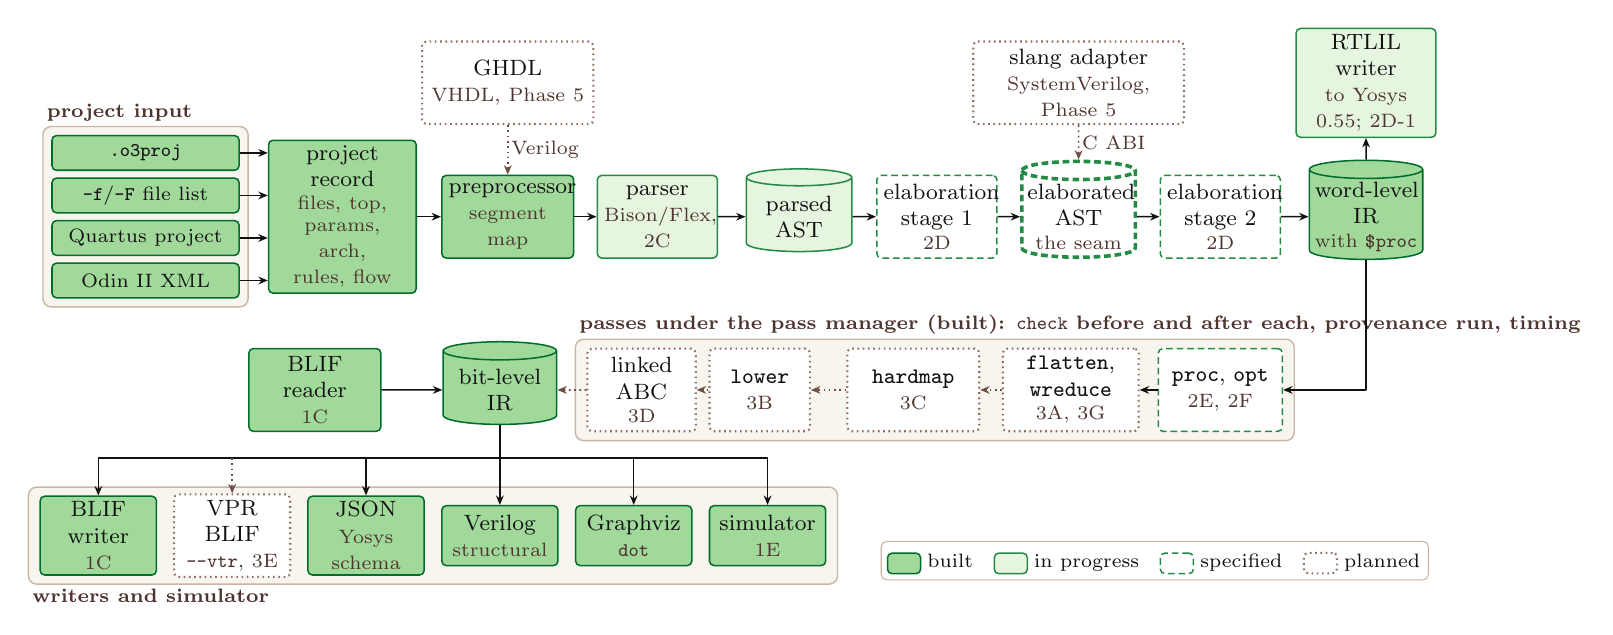
\begin{tikzpicture}[odin, node distance=3mm,
  box/.append style={minimum height=10.5mm}, store/.append style={minimum height=10.5mm}]
  % ---- row 1: project input and the Verilog front end ----------------------------------
  \begin{scope}[every node/.append style={box, built, font=\scriptsize,
                text width=22mm, minimum height=4.4mm, inner ysep=1pt}]
    \node (o3proj) at (1.45, 0.81)  {\odintt{.o3proj}};
    \node (flist)  at (1.45, 0.27)  {\odintt{-f}/\odintt{-F} file list};
    \node (qsf)    at (1.45, -0.27) {Quartus project};
    \node (odin2)  at (1.45, -0.81) {Odin~II XML};
  \end{scope}
  \node[box, built, text width=17mm] (record) at (3.95, 0)
       {project record\\\odinsub{files, top, params,\\arch, rules, flow}};
  \node[box, built, text width=15mm] (pp) at (6.05, 0) {preprocessor\\\odinsub{segment map}};
  \node[box, inprog, text width=13.5mm] (parser) at (7.95, 0) {parser\\\odinsub{Bison/Flex, 2C}};
  \node[store, inprog, text width=12mm] (past) at (9.75, 0) {parsed\\AST};
  \node[box, spec, text width=13.5mm] (st1) at (11.5, 0) {elaboration\\stage 1\\[-1pt]\odinsub{2D}};
  \node[store, spec, emph, text width=13mm] (east) at (13.3, 0) {elaborated\\AST\\[-1pt]\odinsub{the seam}};
  \node[box, spec, text width=13.5mm] (st2) at (15.1, 0) {elaboration\\stage 2\\[-1pt]\odinsub{2D}};
  \node[store, built, text width=13mm] (wir) at (16.95, 0)
       {word-level\\IR\\[-1pt]\odinsub{with \odintt{\$proc}}};

  % ---- row 0: other front ends and the Yosys bridge -----------------------------------
  \node[box, planned, text width=20mm] (ghdl) at (6.05, 1.7)
       {GHDL\\\odinsub{VHDL, Phase 5}};
  \node[box, planned, text width=25mm] (slang) at (13.3, 1.7)
       {slang adapter\\\odinsub{SystemVerilog, Phase 5}};
  \node[box, inprog, text width=16mm] (rtlil) at (16.95, 1.7)
       {RTLIL writer\\\odinsub{to Yosys 0.55; 2D-1}};

  % ---- row 2: passes (right to left) ----------------------------------------------------
  \node[box, spec, text width=14mm] (procopt) at (15.1, -2.2) {\odintt{proc}, \odintt{opt}\\\odinsub{2E, 2F}};
  \node[box, planned, text width=15.5mm] (flat) at (13.2, -2.2)
       {\odintt{flatten},\\\odintt{wreduce}\\[-1pt]\odinsub{3A, 3G}};
  \node[box, planned, text width=15mm] (hmap) at (11.2, -2.2) {\odintt{hardmap}\\\odinsub{3C}};
  \node[box, planned, text width=11mm] (lower) at (9.25, -2.2) {\odintt{lower}\\\odinsub{3B}};
  \node[box, planned, text width=12mm] (abc) at (7.75, -2.2) {linked\\ABC\\[-1pt]\odinsub{3D}};
  \node[store, built, text width=13mm] (bir) at (5.95, -2.2) {bit-level\\IR};
  \node[box, built, text width=15mm] (rblif) at (3.6, -2.2) {BLIF reader\\\odinsub{1C}};

  % ---- row 3: writers and the simulator -------------------------------------------------
  \begin{scope}[every node/.append style={box, text width=13mm, minimum height=7.6mm}]
    \node[built]   (wblif) at (0.85, -4.05) {BLIF writer\\\odinsub{1C}};
    \node[planned] (wvtr)  at (2.55, -4.05) {VPR BLIF\\\odinsub{\odintt{--vtr}, 3E}};
    \node[built]   (wjson) at (4.25, -4.05) {JSON\\\odinsub{Yosys schema}};
    \node[built]   (wver)  at (5.95, -4.05) {Verilog\\\odinsub{structural}};
    \node[built]   (wdot)  at (7.65, -4.05) {Graphviz\\\odinsub{\odintt{dot}}};
    \node[built]   (sim)   at (9.35, -4.05) {simulator\\\odinsub{1E}};
  \end{scope}

  % ---- edges ----------------------------------------------------------------------------
  \foreach \n in {o3proj, flist, qsf, odin2}
    \draw[flow] (\n.east) -- (\n.east -| record.west);
  \draw[flow] (record) -- (pp);
  \draw[flow] (pp) -- (parser);
  \draw[flow] (parser) -- (past);
  \draw[flow] (past) -- (st1);
  \draw[flow] (st1) -- (east);
  \draw[flow] (east) -- (st2);
  \draw[flow] (st2) -- (wir);
  \draw[flowplanned] (ghdl) -- node[edgelabel, right, fill=none] {Verilog} (pp);
  \draw[flowplanned] (slang) -- node[edgelabel, right, fill=none] {C ABI} (east);
  \draw[flow] (wir) -- (rtlil);
  \draw[flow] (wir.south) |- (procopt.east);
  \draw[flow] (procopt) -- (flat);
  \draw[flowplanned] (flat) -- (hmap);
  \draw[flowplanned] (hmap) -- (lower);
  \draw[flowplanned] (lower) -- (abc);
  \draw[flowplanned] (abc) -- (bir);
  \draw[flow] (rblif) -- (bir);
  % bus from the bit-level IR to the writers
  \coordinate (rail) at ($(bir.south)+(0,-0.42)$);
  \draw[line width=0.55pt, draw=o3ink] (bir.south) -- (rail);
  \draw[line width=0.55pt, draw=o3ink] (rail -| wblif) -- (rail -| sim);
  \foreach \n in {wblif, wjson, wver, wdot, sim}
    \draw[flow] (rail -| \n) -- (\n.north);
  \draw[flowplanned] (rail -| wvtr) -- (wvtr.north);

  % ---- regions (background) -------------------------------------------------------------
  \begin{scope}[on background layer]
    \node[region, fit=(o3proj)(odin2), inner xsep=3pt, inner ysep=3pt,
          label={[regionlabel, anchor=south west]north west:project input}] (rin) {};
    \node[region, fit=(procopt)(abc), inner ysep=3pt,
          label={[regionlabel, anchor=south west]north west:{passes under the pass manager
          (built): \odintt{check} before and after each, provenance run, timing}}]
          (rpm) {};
    \node[region, fit=(wblif)(sim), inner ysep=3pt,
          label={[regionlabel, anchor=north west]south west:writers and simulator}] (rout) {};
  \end{scope}

  \odinlegend{anchor=south east, at={(17.75, -4.62)}}
\end{tikzpicture}
}
\caption{The Odin III pipeline and its status on 2026-10-19. Built: merged on the main branch;
in progress: being implemented (linked ABC, whose BLIF exchange is built and whose in-memory
exchange awaits its default flip, and the QoR harness, whose exit runs are open); planned: later
work. Every step inside the core is a pass registered with the pass manager, which runs
\code{check} before and after each pass in Debug builds. The elaborated AST is the seam where a
slang adapter would enter; that adapter and GHDL are deferred (D10). Phase~4's
\code{partial\_map} generalises Phase~3's fixed \code{hardmap}.}
\label{fig:pipeline}
\end{figure*}

Odin III reads a design into one IR and changes that IR one pass at a time. Figure~\ref{fig:pipeline}
shows the whole system and its status (DESIGN \S3, \S6). Figure~\ref{fig:flow} shows the path of
a Verilog design through the stages, in the order of the production script. That script is the O
leg of the \code{vtr-qor} harness (Sec.~\ref{sec:harness}):
\begin{lstlisting}
read_techlib lib/vtr.o3lib
read_verilog --nolatches --vtr-compat d.v
proc; fsm; opt; flatten; wreduce
hardmap; lower
abc --lut 6
write_blif --vtr d.blif
\end{lstlisting}
Here \code{hardmap} is the script name of \code{partial\_map}. A test harness,
\code{hardmap-diff}, runs a longer script that adds \code{opt -full} and \code{opt\_clean} calls
between these passes so that each stage can be compared with Parmys.

\begin{figure*}[t]
\centering
\odinfit{\textwidth}{% The Odin III flow with what each stage does (see fig_flow_base.tex). Wide: \textwidth.
\def\flowbandA{Verilog files, include paths, defines, top, parameters, and the architecture and
  rules: one project record.}%
\def\flowbandB{Preprocessor with a segment map; Bison/Flex parser builds the AST; the symbol
  table maps each name to its declaration, per scope.}%
\def\flowbandC{None. Stage 1 of elaboration evaluates parameters, \odintt{generate} and constant
  functions, because the language requires it. The script runs no \odintt{opt} before \odintt{proc}.}%
\def\flowbandD{Stage 1: elaborated AST (the seam). Stage 2: bind names, widths, word cells;
  \odintt{always} becomes a \odintt{\$proc} cell. \odintt{proc}: muxes, latches, flip-flops.}%
\def\flowbandE{\odintt{fsm}: find and recode state machines. \odintt{opt}: \odintt{opt\_expr}
  folds constants; \odintt{opt\_clean} removes dead cells; \odintt{opt\_merge} merges equal cells;
  \odintt{opt\_share} shares operators. \odintt{flatten}: inline instances. \odintt{wreduce}: narrow widths.}%
\def\flowbandF{Binds \odintt{\$mul}, \odintt{\$add}/\odintt{\$sub} and \odintt{\$mem} to the hard
  blocks the arch record lists: multipliers, adder chains, RAM. The rest stays soft.}%
\def\flowbandG{Every word cell becomes bit cells; flip-flops become \odintt{\$\_DFF\_P\_}; a
  leftover \odintt{\$mem} becomes flip-flops and muxes.}%
\def\flowbandH{Linked ABC optimises the soft logic as an AIG and maps it to $K$-input LUTs,
  one run per clock domain. Hard cells are cut points.}%
\def\flowbandI{BLIF \odintt{--vtr} for VPR; structural Verilog; Yosys JSON; LPM Verilog for
  Quartus; Graphviz \odintt{dot}; RTLIL to Yosys.}%
\def\flowbandJ{Each output can be read back with its HDL locations: \odintt{read\_blif},
  \odintt{read\_verilog -icells}, \odintt{read\_json}.}%
% The Odin III flow, drawn once (the O leg of tools/vtr-qor, qor_legs.py, plus the readers of
% Phase 5). Nine stages in two rows, a band of text under each box. The three figures that use it
% (fig_flow, fig_flow_verify, fig_flow_prov) define \flowbandA ... \flowbandJ, the text of each
% band, and then input this file. Wide figure: \textwidth.
\begin{tikzpicture}[odin,
  st/.style={box, built, text width=29.5mm, minimum height=13mm, inner ysep=2pt},
  band/.style={font=\scriptsize, text width=29.5mm, align=left, anchor=north, inner sep=1.2pt,
               color=o3ink}]
  % ---- row 1 ---------------------------------------------------------------------------
  \node[st] (s1) at (0, 0) {\textbf{Code}\\[-1pt]\odinsub{Verilog and the project}};
  \node[st] (s2) at (3.4, 0) {\textbf{Parse}\\[-1pt]\odinsub{\odintt{read\_verilog}: AST and symbol table}};
  \node[st, planned] (s3) at (6.8, 0) {\textbf{Before elaboration}\\[-1pt]\odinsub{no optimisation pass}};
  \node[st] (s4) at (10.2, 0) {\textbf{Elaborate}\\[-1pt]\odinsub{stage 1, stage 2, \odintt{proc}}};
  \node[st] (s5) at (13.6, 0) {\textbf{Word-level passes}\\[-1pt]\odinsub{\odintt{fsm}, \odintt{opt}, \odintt{flatten}, \odintt{wreduce}}};
  % ---- row 2 ---------------------------------------------------------------------------
  \node[st] (s6) at (0, -5.4) {\textbf{Partial mapping}\\[-1pt]\odinsub{\odintt{partial\_map} (\odintt{hardmap}) on the arch record}};
  \node[st] (s7) at (3.4, -5.4) {\textbf{Lower}\\[-1pt]\odinsub{\odintt{lower}: words to bits}};
  \node[st] (s8) at (6.8, -5.4) {\textbf{Logic and LUTs}\\[-1pt]\odinsub{linked ABC: \odintt{abc --lut K}}};
  \node[st] (s9) at (10.2, -5.4) {\textbf{Outputs}\\[-1pt]\odinsub{\odintt{write\_blif --vtr}, Verilog, JSON, LPM, dot}};
  \node[st, spec] (s10) at (13.6, -5.4) {\textbf{Read back}\\[-1pt]\odinsub{BLIF, Verilog, JSON readers (Phase 5)}};
  % ---- bands ---------------------------------------------------------------------------
  \foreach \i/\t in {1/\flowbandA, 2/\flowbandB, 3/\flowbandC, 4/\flowbandD, 5/\flowbandE,
                     6/\flowbandF, 7/\flowbandG, 8/\flowbandH, 9/\flowbandI, 10/\flowbandJ}
    \node[band] at ([yshift=-1.4mm]s\i.south) {\t};
  % ---- edges ---------------------------------------------------------------------------
  \foreach \a/\b in {s1/s2, s2/s3, s3/s4, s4/s5, s6/s7, s7/s8, s8/s9}
    \draw[flow] (\a) -- (\b);
  \draw[flow] (s5.east) -- ++(0.4,0) |- (0,-4.4) -- (s6.north);
  \draw[ref] (s9) -- (s10);
\end{tikzpicture}

}
\caption{The flow of a Verilog design through Odin III, in the order of the production script.
Each box is a stage; the text under it says what it does. The dotted box marks a stage that does
nothing, and the dashed box a stage that is specified but not yet built. Every stage from
\code{proc} to \code{write\_blif} is a registered pass.}
\label{fig:flow}
\end{figure*}

The stages come from four tools, and each idea keeps its lineage. From Odin and Odin~II, Odin III
takes the node, pin and net model, the Bison and Flex parser, the reading of an architecture file
and the idea of partial mapping. From Yosys, it takes the word-level cell set and the semantics of
Verilog elaboration, and it re-implements the \code{proc}, \code{opt}, \code{wreduce},
\code{fsm}, \code{flatten} and \code{techmap} steps in C. From Parmys, it takes the order of the
script and the hard-block rules for the VTR architecture. From ABC, it takes logic optimisation
and LUT mapping, linked into the core.

\emph{Parse.} A project (Sec.~\ref{sec:project}) names the files. The preprocessor and the parser
build a parsed AST with source locations, and the symbol table records each declaration
(Phase~2; Sec.~\ref{sec:parser}).

\emph{Before elaboration.} Odin III has no optimisation pass here. Yosys simplifies its AST before
\code{genrtlil}; Odin III does not. Elaboration stage~1 evaluates parameters, \code{generate} blocks and
constant functions, because the language fixes their values. A pre-\code{proc} \code{opt}, as
Parmys runs, is possible because the \code{opt} passes accept \code{\$proc} cells, but the
production script does not run it (PHASE4 decision 14, item~5).

\emph{Elaborate.} Two stages through an elaborated AST give word-level IR in which each
\code{always} block is a \code{\$proc} cell (Sec.~\ref{sec:seam}). \code{proc} then turns these
cells into mux trees, latches and flip-flops, step by step as Yosys's \code{proc\_*} passes do.

\emph{Word-level passes.} \code{fsm} finds state machines and recodes them one-hot, as Yosys's
\code{fsm} does, placed right after \code{proc} as Parmys places it. \code{opt} is Yosys's
\code{opt} family: \code{opt\_expr} folds constants, \code{opt\_clean} removes dead cells,
\code{opt\_merge} merges cells with equal inputs, \code{opt\_share} merges operators that feed the
same mux, and \code{opt\_muxtree}, \code{opt\_reduce} and \code{opt\_dff} tidy
muxes, reductions and flip-flops. \code{flatten} inlines the instances, and \code{wreduce}
narrows widths. The paragraphs below describe them.

\emph{Partial mapping.} Following Odin~II's partial mapping and Parmys's hard-block rules,
\code{partial\_map} binds word-level multipliers, adders and RAMs to the hard blocks that the
architecture record lists, and leaves the rest soft (Sec.~\ref{sec:hardmap}).

\emph{Lower, logic and LUTs.} \code{lower} takes every word cell to bits. The linked ABC
optimises the soft logic and maps it to $K$-input LUTs, with VTR's own script as the default.

\emph{Outputs.} BLIF with \code{--vtr} goes to VPR. Verilog, Yosys-schema JSON and LPM Verilog for
Quartus, Graphviz \code{dot} and RTLIL go to other tools. Sections~\ref{sec:backend} to
\ref{sec:harness} describe the Phase~3 stages, and Sec.~\ref{sec:features} lists every feature
with its phase and status.

\subsection{One IR, two granularities, passes everywhere}

There is one IR (ADR D1). Each cell type carries a granularity tag---\code{word},
\code{bit}, \code{hard}, \code{blackbox}, plus the structural \code{module} and
\code{port}---and two \emph{views} are assertions over that tag: the RTLIL view admits word,
hard and black-box cells; the netlist view admits bit, hard and black-box cells; mixed
granularity is legal only inside \code{lower} and \code{raise} (IR-9). Every reader, writer,
checker, the simulator and the matcher therefore exist once.

Every reader, writer and transformation is a pass. Running a pass opens a provenance pass run,
runs the full structural \code{check} before and after it in Debug builds (or with
\code{--check} in Release), times it and logs it (1D spec). Since 2D-1 a pass also declares
whether it handles processes, and refusal is the default (EL-33). The eight \code{opt} passes
accept them and treat \code{\$proc} as opaque, so Parmys's pre-\code{proc} optimisations run in
Parmys's order (``mode~P''; the order changes netlists: 812 against 792 cells on
\code{stereovision3}); every other pass refuses a design that still holds \code{\$proc} cells.

\subsection{Project input}
\label{sec:project}

\begin{figure}[t]
\centering
\odinfit{\columnwidth}{% Project input (DESIGN.md section 4.0, 2B spec PRJ-1..PRJ-18): every format fills one
% design-owned project record; read_verilog, the tech library, dump_project and (Phase 4) the
% partial mapper only read it. Single column: \columnwidth.
\begin{tikzpicture}[odin,
  fmt/.style={box, built, text width=18mm, minimum height=10.5mm},
  use/.style={box, text width=18.4mm, minimum height=11mm, inner xsep=1.5pt},
  fld/.style={draw=o3grey6, fill=white, line width=0.5pt, font=\scriptsize, align=left,
              text width=40mm, minimum height=5.6mm, inner xsep=2.2pt, inner ysep=1pt},
  fldh/.style={fld, fill=o3blue4, draw=o3blue8, font=\footnotesize, align=center,
               text width=80mm+3.9pt, minimum height=5mm}]
  % ---- the four formats --------------------------------------------------------------------
  \foreach \n/\x/\t/\s in {
      o3/1.05/\odintt{.o3proj}/{native; arch,\\rules and flow},
      fl/3.25/file list/{EDA style:\\\odintt{-f}, \odintt{-F}},
      qs/5.45/Quartus/{\odintt{.qpf}, \odintt{.qsf},\\\odintt{.qip}},
      ox/7.65/Odin~II XML/{the \odintt{config}\\file}}
    \node[fmt] (\n) at (\x, 0) {\t\\\odinsub{\s}};

  % ---- the record: a header and two columns of fields ---------------------------------------
  \node[fldh] (rh) at (4.35, -1.45) {project record \odinsub{(design-owned; 2B)}};
  \node[fld, anchor=north west] (f1) at ($(rh.south west)+(0,\pgflinewidth)$)
       {files: path as given and resolved, location, language, library};
  \node[fld, anchor=north west] (f3) at ($(f1.south west)+(0,\pgflinewidth)$)
       {top and its location; params \odintt{scope.name = value}};
  \node[fld, anchor=north west] (f5) at ($(f3.south west)+(0,\pgflinewidth)$)
       {mapping rules: \odintt{map}, \odintt{split}, \odintt{limit}, patterns (stored)};
  \node[fld, anchor=north west] (f7) at ($(f5.south west)+(0,\pgflinewidth)$)
       {flow script; ignored keys; duplicates};
  \node[fld, anchor=north west] (f2) at ($(f1.north east)+(-\pgflinewidth,0)$)
       {library files and directories, \odintt{libext}, include directories, defines};
  \node[fld, anchor=north west] (f4) at ($(f2.south west)+(0,\pgflinewidth)$)
       {architecture: \odintt{.o3lib}, VPR XML or device};
  \node[fld, anchor=north west] (f6) at ($(f4.south west)+(0,\pgflinewidth)$)
       {inventory (\odintt{available}); overrides (\odintt{hide}, \odintt{cell from})};
  \node[fld, anchor=north west] (f8) at ($(f6.south west)+(0,\pgflinewidth)$)
       {revision; output (Odin~II XML)};
  \node[fit=(rh)(f1)(f8), inner sep=0pt, draw=o3blue8, line width=0.7pt] (rec) {};

  % ---- the readers of the record ------------------------------------------------------------
  \node[use, inprog]  (rv) at (1.05, -5.0) {{\scriptsize\odintt{read\_verilog}}\\\odinsub{preprocess, parse,\\[-2pt]elaborate}};
  \node[use, built]   (rt) at (3.25, -5.0) {{\scriptsize\odintt{read\_techlib}}\\\odinsub{\odintt{.o3lib}, 1G}};
  \node[use, planned] (pm) at (5.45, -5.0) {{\scriptsize\odintt{partial\_map}}\\\odinsub{Phase 4}};
  \node[use, built]   (dp) at (7.65, -5.0) {{\scriptsize\odintt{dump\_project}}\\\odinsub{JSON: the corpus\\[-2pt]oracle record}};

  \foreach \n in {o3, fl, qs, ox} \draw[flow] (\n.south) -- (\n.south |- rec.north);
  \foreach \n in {rv, rt, dp}     \draw[flow] (\n.north |- rec.south) -- (\n.north);
  \draw[flowplanned] (pm.north |- rec.south) -- (pm.north);

  \odinlegend{anchor=north, at={(4.35, -5.75)}}
\end{tikzpicture}
}
\caption{Project input: four formats fill one design-owned record, which every reader shares.
Mapping rules, inventory and overrides are read and stored in Phase~2; interpreting the
mapping rules is not in v1.0 (D10).}
\label{fig:project}
\end{figure}

A design reaches Odin III as one project record that every reader shares
(Fig.~\ref{fig:project}; DESIGN \S4.0). It holds the source files with language and library,
include paths and defines, the top and its parameter overrides, and---unusually for a
synthesis front end---the \emph{architecture} and \emph{partial-mapping rules}: tech libraries
or architecture files, a per-cell inventory (\code{available multiply 112}), research overrides
(\code{hide} a cell, a variant \code{cell ... from ...}), scoped mapping rules with thresholds
and budgets, and optionally the flow script, so that one file reproduces a run:

\begin{lstlisting}
file verilog rtl/top.v
incdir rtl/include
define WIDTH=8
top top
param top.WIDTH 16
arch k6_frac_N10_mem32K.o3lib
map * $mul to multiply min_width 9
limit multiply 40
flow synth.o3
\end{lstlisting}

The same record is filled from an EDA file list (\code{-f}/\code{-F}, \code{+incdir+},
\code{+define+}, \code{-v}/\code{-y}) or a Quartus \code{.qpf}/\code{.qsf}/\code{.qip} project,
whose synthesis assignments (\code{AUTO\_DSP\_RECOGNITION}, \code{MULTSTYLE}, \ldots) become
mapping rules. Rule precedence is source attribute, instance path, module, global, then
architecture default. The rules are read, checked and stored today; a mapper that interprets
them would record the rule (file and line) that chose each binding in provenance, but that
mapper is not in v1.0 (D10, PHASE4 4.11). Unknown keys are errors, so a typo never silently changes a
mapping. The grammar of all formats is normative in DESIGN \S4.0 and pinned by a corpus of 55
project cases (36 positive, 19 negative), each written in every format that can express it,
with a stdlib Python reference parser as the oracle for the C readers.

\subsection{Two-stage elaboration and the seam}
\label{sec:seam}

\begin{figure*}[t]
\centering
\odinfit{\textwidth}{% Two-stage elaboration with the elaborated AST as the seam (2D spec section 2, EL-2, EL-4).
% Stage 1 is Verilog-only; stage 2 is shared by every front end. The slang adapter (Phase 5)
% builds the elaborated form through the C ABI and enters at stage 2. Wide: \textwidth.
\begin{tikzpicture}[odin,
  stage/.style={box, text width=34mm, align=left, minimum height=21mm},
  list/.style={font=\scriptsize, align=left}]
  % ---- the main row ------------------------------------------------------------------------
  \node[box, neutral, text width=15mm, minimum height=12mm] (vf) at (0.95, 0)
       {Verilog-2005\\files\\[-1pt]\odinsub{preprocessed, 2B}};
  \node[store, built, text width=14mm, minimum height=14mm] (ps) at (2.95, 0)
       {parsed\\store\\[-1pt]\odinsub{form \odintt{PARSED}}\\[-2pt]\odinsub{2C}};
  \node[stage, inprog] (s1) at (5.84, 0)
       {\textbf{stage 1} (Verilog only)\\[1pt]
        \scriptsize module lookup, top selection\\
        \scriptsize \odintt{\#()}, \odintt{defparam}, project params\\
        \scriptsize specialisation\\
        \scriptsize \odintt{generate}\\
        \scriptsize constant functions\\
        \scriptsize implicit nets};
  \node[store, spec, emph, text width=30mm, inner xsep=4pt, inner ysep=0pt, minimum height=20mm] (es) at (9.81, 0)
       {\textbf{elaborated store}\\[-1pt]\odinsub{the seam, form}\\[-2pt]\odinsub{\odintt{ELABORATED}}\\[1pt]
        \scriptsize no \odintt{generate} or \odintt{defparam}\\
        \scriptsize constants resolved\\
        \scriptsize one \odintt{MODULE} per\\
        \scriptsize specialisation};
  \node[stage, spec] (s2) at (13.78, 0)
       {\textbf{stage 2} (every front end)\\[1pt]
        \scriptsize binding (symbol table)\\
        \scriptsize Yosys widths and signedness\\
        \scriptsize word cells, drivers, \odintt{\$mem}\\
        \scriptsize \odintt{always} $\rightarrow$ \odintt{\$proc} cells\\
        \scriptsize inlining, initial values};
  \node[store, built, text width=16mm, minimum height=14mm] (ir) at (16.94, 0)
       {word-level\\IR\\[-1pt]\odinsub{+ \odintt{\$proc} (2D-1)}};

  % ---- around the seam -----------------------------------------------------------------------
  \node[box, light, text width=40mm, align=center] (chk) at (9.81, 2.0)
       {\odintt{odin3\_ast\_check}, rule 7\\\odinsub{enforces the elaborated subset}};
  \node[box, planned, text width=36mm] (sl) at (9.81, -2.35)
       {slang adapter (C++)\\\odinsub{\odintt{odin3\_ast\_*} builders; Phase 5}};
  \node[box, built, text width=19.5mm] (rt) at (16.94, -2.35)
       {\odintt{write\_rtlil}\\\odinsub{2D-1}};
  \node[box, external, text width=28mm] (yo) at (13.6, -2.35)
       {Yosys 0.55 (Parmys's)\\\odinsub{equivalence oracle}};

  % ---- edges ---------------------------------------------------------------------------------
  \draw[flow] (vf) -- (ps);
  \draw[flow] (ps) -- (s1);
  \draw[flow] (s1) -- (es);
  \draw[flow] (es) -- (s2);
  \draw[flow] (s2) -- (ir);
  \draw[flow] (ir) -- (rt);
  \draw[flow] (rt) -- (yo);
  \draw[flowplanned] (sl) -- node[edgelabel, right] {\odintt{odin3\_ast\_elaborate} (C ABI)} (es);
  \draw[line width=0.5pt, draw=o3blue7, dash pattern=on 2.4pt off 1.4pt] (chk) -- (es);

  % ---- regions -------------------------------------------------------------------------------
  \begin{scope}[on background layer]
    \node[region, fit=(vf)(ps)(s1), inner sep=5pt,
          label={[regionlabel, anchor=south west]north west:stage 1: Verilog-specific}] {};
    \node[region, fit=(s2)(ir), inner sep=5pt,
          label={[regionlabel, anchor=south east]north east:stage 2: shared by every front end}] {};
  \end{scope}

  \odinlegend{anchor=west, at={(0.0, -2.35)}}
\end{tikzpicture}
}
\caption{Two-stage elaboration (2D spec). Stage~1 is Verilog-only and produces an elaborated
AST; stage~2 is shared by every front end. The slang adapter builds the elaborated form through
the C ABI and enters at stage~2. \code{write\_rtlil} hands the result to Parmys's Yosys~0.55 for
equivalence checking.}
\label{fig:seam}
\end{figure*}

Elaboration is split at an \emph{elaborated AST} (Fig.~\ref{fig:seam}; PHASE2 \#8 Q3, 2D
EL-2). Stage~1 is Verilog-specific: module lookup, top selection, parameter overrides
(\code{\#()}, \code{defparam}, project \code{param}), specialisation, \code{generate} and
constant functions. Its output is a second AST store in the same format, restricted to a
subset that \code{odin3\_ast\_check} enforces: no generate constructs or \code{defparam}, every
range and parameter a constant leaf, one \code{MODULE} per parameter specialisation, generate
scopes named with their indices. Stage~2 is language-neutral: binding through the symbol table,
widths and signedness, word cells, drivers, memories, processes, inlining and initial values.

The seam exists for SystemVerilog. slang already elaborates SV; its adapter (a small C++ shim,
the only C++ outside \code{third\_party}) would emit the elaborated subset through the C ABI and
call stage~2. That adapter is deferred (D10), but the seam is built. Without it, Phase~5 would need a second elaborator over slang's output and
the two would drift. VHDL takes a different path, \code{ghdl --synth} to Verilog
(ADR D2).

Stage~2 represents an \code{always} block as a \code{\$proc} cell: a word-level node whose
\code{I} pins are every net the process reads and whose \code{O} pins are every net it drives,
with Yosys's decision structure (switches, cases, actions, syncs) stored as an opaque, validated
parameter whose positions are pin indices (EL-33). Because the connectivity is ordinary pins,
every IR invariant, driver query and fanout walk holds unchanged; a first design that referenced
nets by ID without pins was rejected in review because it broke the ``every driver is a pin''
rule.

\subsection{Parsing}
\label{sec:parser}

The parser (2C; PHASE2 \#10, \#15) keeps Odin~II's Bison/Flex lineage but not its grammar. A
reentrant Flex lexer reads the preprocessor's stream, and a pure LALR(1) Bison grammar
(\code{\%expect 0}, no \code{\%expect-rr}) has no reported conflicts in its 947 states. The
conflicts that Bison resolves by precedence must equal a committed allowlist (731 lines: the
operator pairs and the dangling \code{else}), so a grammar change cannot silently add one.
Precedence follows IEEE~1364 Table~5-4, and every binary operator is left-associative,
\code{**} included, as in Yosys (Odin~II makes \code{**} right-associative). Error recovery
resynchronises at \code{;} and \code{endmodule}, and stops after 20 errors. The Bison and Flex
output is generated at build time, never committed, and compiled inside the core under one
per-file warning flag.

Each parse is checked twice. \code{odin3-parse-check} runs a \emph{location oracle}: every
node's first token must spell the node, its range must end on a token end, and children must
lie inside their parents. It also prints the tree, parses the text again and requires equal
trees. Two independent generators of input go further. A libFuzzer target feeds raw bytes and
token streams with allocation failures injected and every cap lowered, and requires either a
clean tree or 1--20 located errors; about 62,000 raw-mode runs found one bug, a backslash before
a NUL byte in a string, now fixed. A random-module generator covers the coverage audit's
required and recommended rows. It prints with minimal parentheses from its own copy of
Table~5-4 and dumps its own tree, so it is an oracle independent of the parser. Each seed is
classified against Yosys~0.55, and Odin III must reproduce the generator's tree (200 seeds in
CTest).

\subsection{Processes: \code{proc}}

\begin{figure}[t]
\centering
\odinfit{\columnwidth}{% The proc pass (2E spec sections 2.1-2.2, PR-2/PR-3): Yosys 0.55's proc -norom sub-passes as
% internal phases of one pass, per module. Step A analyses every process of a module without
% changing the IR; steps B-F lower it only if no process of the module has an error, so a module
% is lowered completely or not at all. Each box: 2E's phase, the Yosys 0.55 sub-pass it mirrors,
% and what it does. Single column: \columnwidth.
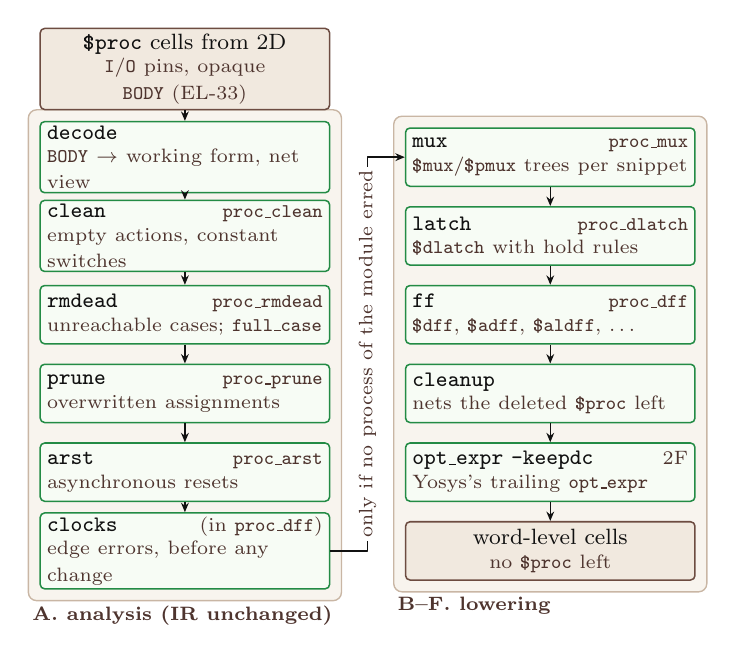
\begin{tikzpicture}[odin,
  ph/.style={box, light, text width=35mm, align=left, minimum height=7.4mm, inner ysep=1.4pt}]
  % ---- input ---------------------------------------------------------------------------------
  \node[box, neutral, text width=35mm] (in) at (1.98, 1.12)
       {\odintt{\$proc} cells from 2D\\[-1pt]\odinsub{\odintt{I}/\odintt{O} pins, opaque \odintt{BODY} (EL-33)}};
  % ---- step A: analysis --------------------------------------------------------------------------
  \node[ph] (dec) at (1.98, 0)
       {\odintt{decode}\\[-1pt]\odinsub{\odintt{BODY} $\to$ working form, net view}};
  \node[ph] (cln) at (1.98, -1.0)
       {\odintt{clean}\hfill{\scriptsize\color{o3sub}\odintt{proc\_clean}}\\[-1pt]\odinsub{empty actions, constant switches}};
  \node[ph] (rmd) at (1.98, -2.0)
       {\odintt{rmdead}\hfill{\scriptsize\color{o3sub}\odintt{proc\_rmdead}}\\[-1pt]\odinsub{unreachable cases; \odintt{full\_case}}};
  \node[ph] (prn) at (1.98, -3.0)
       {\odintt{prune}\hfill{\scriptsize\color{o3sub}\odintt{proc\_prune}}\\[-1pt]\odinsub{overwritten assignments}};
  \node[ph] (ars) at (1.98, -4.0)
       {\odintt{arst}\hfill{\scriptsize\color{o3sub}\odintt{proc\_arst}}\\[-1pt]\odinsub{asynchronous resets}};
  \node[ph] (clk) at (1.98, -5.0)
       {\odintt{clocks}\hfill{\scriptsize\color{o3sub}(in \odintt{proc\_dff})}\\[-1pt]\odinsub{edge errors, before any change}};
  % ---- steps B-F: lowering -------------------------------------------------------------------
  \node[ph] (mux) at (6.62, 0)
       {\odintt{mux}\hfill{\scriptsize\color{o3sub}\odintt{proc\_mux}}\\[-1pt]\odinsub{\odintt{\$mux}/\odintt{\$pmux} trees per snippet}};
  \node[ph] (lat) at (6.62, -1.0)
       {\odintt{latch}\hfill{\scriptsize\color{o3sub}\odintt{proc\_dlatch}}\\[-1pt]\odinsub{\odintt{\$dlatch} with hold rules}};
  \node[ph] (dff) at (6.62, -2.0)
       {\odintt{ff}\hfill{\scriptsize\color{o3sub}\odintt{proc\_dff}}\\[-1pt]\odinsub{\odintt{\$dff}, \odintt{\$adff}, \odintt{\$aldff}, \ldots}};
  \node[ph] (cup) at (6.62, -3.0)
       {\odintt{cleanup}\\[-1pt]\odinsub{nets the deleted \odintt{\$proc} left}};
  \node[ph, light] (opt) at (6.62, -4.0)
       {\odintt{opt\_expr -keepdc}\hfill{\scriptsize\color{o3sub}2F}\\[-1pt]\odinsub{Yosys's trailing \odintt{opt\_expr}}};
  \node[box, neutral, text width=35mm, minimum height=7.4mm] (out) at (6.62, -5.0)
       {word-level cells\\[-1pt]\odinsub{no \odintt{\$proc} left}};

  % ---- edges ---------------------------------------------------------------------------------
  \draw[flow] (in) -- (dec);
  \foreach \a/\b in {dec/cln, cln/rmd, rmd/prn, prn/ars, ars/clk, mux/lat, lat/dff, dff/cup,
                     cup/opt, opt/out}
    \draw[flow] (\a) -- (\b);
  \coordinate (bus) at (4.30, 0);
  \draw[flow] (clk.east) -- (clk.east -| bus) -- (bus) -- (mux.west);
  \node[font=\scriptsize, color=o3sub, rotate=90, fill=white, inner sep=1pt]
       at ($(bus)!0.5!(clk.east -| bus)$) {only if no process of the module erred};

  % ---- regions -------------------------------------------------------------------------------
  \begin{scope}[on background layer]
    \node[region, fit=(dec)(clk), inner sep=4pt,
          label={[regionlabel, anchor=north west]south west:A. analysis (IR unchanged)}] {};
    \node[region, fit=(mux)(out), inner sep=4pt,
          label={[regionlabel, anchor=north west]south west:B--F. lowering}] {};
  \end{scope}
\end{tikzpicture}
}
\caption{The \code{proc} pass (2E spec \S2): Yosys~0.55's \code{proc -norom} sub-passes, as
Parmys runs them, as phases of one pass in Yosys's order. Each box shows 2E's phase, the
Yosys sub-pass it mirrors, and what it does. Step~A changes nothing; a module is lowered only if
none of its processes has an error, so it is lowered completely or not at all. 2E is built
(2E-1 to 2E-3); the trailing \code{opt\_expr} is 2F's, also built.}
\label{fig:proc}
\end{figure}

\code{proc} (2E) turns \code{\$proc} cells into mux trees, latches and flip-flops by
re-implementing Yosys~0.55's \code{proc\_*} sub-passes in C (Fig.~\ref{fig:proc}). Each
process is decoded into a working form over the module's nets. The decision-tree phases
(\code{clean}, \code{rmdead}, \code{prune}, \code{arst}) and a clock pre-check run on every
process of a module before the IR changes; then \code{mux}, \code{latch} and \code{ff} lower
it. The flip-flop phase targets eleven word-level flip-flop and latch cells added with Yosys's
simlib ports (\code{\$adffe} to \code{\$sr}; IR change~D). Every walk that Yosys writes
recursively is an explicit stack, and every unit-test expectation was re-derived by running
Yosys~0.55's sub-passes up to the same phase. \code{proc-diff} gives both tools the same RTLIL
and compares their netlists.

The 2E specification declares 19 divergences from Yosys~0.55 (\S20). Most are for robustness or
determinism. Yosys recurses until its stack overflows on a combinational cycle, and 2E stops
after 1,024 hops or treats the cycle as no feedback. 2E memoises the latch walk, which is
exponential in Yosys on shared cones. It caps pattern pools, and it visits processes in node-ID
order. One divergence is a correctness fix (\S20 \#18, Sec.~\ref{sec:compare}).

\subsection{The back end: the Phase 3 script}
\label{sec:backend}

Phase~3 takes word-level IR to a netlist that VPR places and routes. Its exit test runs the
production script of Sec.~\ref{sec:arch} on the VTR benchmarks of the local gate and routes the
result with VPR (PHASE3 exit item~3). Where Odin III and Parmys could differ,
\code{--vtr-compat} makes Odin III do what Parmys does and print a WARNING when the result still
differs (Sec.~\ref{sec:verify}). The harness \code{hardmap-diff} runs a longer script in Parmys's
order, with \code{wreduce} before \code{flatten} and extra \code{opt -full} calls (PHASE3 \#7,
\#30, \#31), so that the netlist before ABC can be compared. The next five subsections describe
the stages.

\subsection{Word-level optimisation: \code{opt} and \code{fsm}}
\label{sec:opt}

\code{opt} (2F) follows Yosys~0.55's \code{opt} family and runs its sub-passes to a fixed point.
Each sub-pass is a rewrite of the cell graph.
\code{opt\_expr} folds constants and simplifies arithmetic and logic whose inputs are constant or
repeated. \code{opt\_clean} removes cells and wires that reach no output (dead-code removal).
\code{opt\_merge} merges cells of one type with the same inputs (common-subexpression
elimination); with \code{-ffbits} it also merges identical bits of word flip-flops before
\code{lower}, as Yosys does after \code{techmap} (PHASE3 \#49). \code{opt\_share} merges operators
that feed the same mux (PHASE3 \#52). \code{opt\_muxtree} and \code{opt\_reduce} collapse
muxes and reductions, and \code{opt\_dff} removes flip-flop features that are never used. Each
call is checked as a refinement by \code{opt-equiv} (Sec.~\ref{sec:verify}). \code{opt} never
renumbers IDs; the scripts call \code{compact} when they want that.

\code{fsm} (4.8) is Odin III's port of Yosys~0.55's \code{fsm} (\code{fsm\_detect},
\code{fsm\_extract}, \code{fsm\_opt}, \code{fsm\_recode}, \code{fsm\_map}). It finds a state
register and its next-state logic, extracts the state graph, and recodes it. It runs right after
\code{proc}, where Parmys runs it. The \code{fsm\_encoding} attribute is honoured, and
\code{auto} gives one-hot below 32 states and binary from 32. The recoded register and logic get
DERIVED records whose parents are the original register and logic, and each FSM gets attributes
(state count, encoding) for the analysis flow. It is merged.

\subsection{Width reduction and flattening: \code{wreduce} and \code{flatten}}

\code{wreduce} (3G) narrows word cells to the widths their inputs and readers need, as Yosys
0.55's \code{wreduce} does, signed rewrite included, and visits an operand before its consumer as Yosys does (PHASE3 \#51). It matters because widths decide hard-block
counts: an adder chain has one \code{adder} cell per operand bit, and the multiplier threshold
reads operand widths. Without it, CLB and adder counts drift for reasons unrelated to mapping.
Parmys runs it before \code{flatten}; the production script runs it after.

\code{flatten} (3A) turns a design whose top module instantiates other modules into one flat
top module. It expands instances top-down from a worklist. The nets joined at a port become one
net with IR-2 aliases. Every flattened object gets a dotted instance-path name (the separator is
an option), and the path is kept in a DERIVED provenance record (\code{hier}), so the hierarchy
is recoverable after flattening (Sec.~\ref{sec:re}). Black boxes and library cells stay
untouched, and a pre-flight reports recursive instantiation and any exceeded cap before the IR
changes. Its oracle is Yosys~0.55's \code{flatten}, compared by \code{flatten-diff} on names,
widths and cell types and by an equivalence proof (PHASE3 \#30, \#35).

\subsection{Partial mapping: \code{partial\_map}}
\label{sec:hardmap}

\code{partial\_map} is Odin III's partial mapping. The idea is Odin~II's: bind some of the
word-level design to the hard blocks of the target and leave the rest soft for ABC. The rules
follow Parmys. The pass began as the fixed pass \code{hardmap} (3C), which copies Parmys's defaults for the architecture
\code{k6\_frac\_N10\_frac\_chain\_mem32K\_40nm}, whose \code{<models>} are \code{adder},
\code{multiply}, \code{single\_port\_ram} and \code{dual\_port\_ram} (PHASE3 decisions 2, 4).
Library cells come from \code{lib/vtr.o3lib} (1G), not from code. Phase~4 renamed the pass \code{partial\_map} and kept \code{hardmap} as an alias, and the
script of Fig.~\ref{fig:flow} still says \code{hardmap}. Parmys's rule is the default, and every
improvement is a named option that is off by default (PHASE4 decision 12). The k6 rules, which the
architect approved before any code was written, are:
\begin{itemize}
\item \emph{Multipliers.} A \code{\$mul} becomes a \code{multiply} cell of width 36. Low pins
  carry the operand bits and the rest is padded with \code{unconn}. Small multipliers
  ($2\times2$) and wider ones stay soft, with a warning, for \code{lower}.
\item \emph{Adders and subtractors.} A \code{\$add} or \code{\$sub} becomes a chain of
  $\max(A,B)+2$ \code{adder} cells: a head, one stage per bit and a top stage. A subtraction is
  $a+\lnot b+1$.
\item \emph{RAM.} A \code{\$mem} first merges the flip-flops on its ports, then becomes
  \code{single\_port\_ram} or \code{dual\_port\_ram} slices. Memories that cannot share a RAM
  port are replicated or stay soft, with a warning.
\end{itemize}
Nodes are named \code{<cell>.<role>} and carry a \code{hardmap} attribute.

Phase~4 generalises the pass from the architecture record. \code{read\_arch} (4.1) reads the
\code{<models>} and \code{pb\_type}s of a VPR architecture file into a tech library and an
\emph{arch record} on the design. Three pull requests of \code{partial\_map} are merged. PR~A
is the pass shell, the rule table, the alias and an identity gate, which requires the new pass
to give the same netlist as \code{hardmap} on the k6 architecture. PR~B is \code{memory\_merge}
(4.7), which merges registered reads and writes into the ports of a \code{\$mem}; a
\code{ram\_style} attribute is ignored with a warning. PR~C binds generic hard blocks from the
arch record (4.2), matched by exact port signature as in Odin~II. PR~D is in progress. It maps a
RAM with a read enable to the architecture's RAM and emulates the enable exactly in logic,
because the architecture's RAMs have no read-enable pin (PHASE3 decision 56, approved by the
architect on 2026-10-20).

\subsection{Lowering to bits: \code{lower}}

\code{lower} (3B) turns every word cell into bit cells so that the netlist view (IR-9) holds.
It reproduces Yosys~0.55's \code{simplemap} and \code{techmap.v} structures. Each word cell is
one transaction: new bit nodes on fresh nets, one DERIVED provenance record, then the word node
is deleted. The bit nodes are named after their word cell, so a gate can be read back to the
operator it came from (PHASE3 \#38). The flip-flop family becomes \code{\$\_DFF\_P\_} plus
enable and reset logic. Asynchronous resets are made synchronous, as Parmys's \code{adff2dff}
does (PHASE3 \#19; \code{--async sync}, with \code{--async error} to refuse). A falling-edge
flip-flop is inverted by default (\code{--neg-edge invert}) or kept (\code{keep}). A leftover
\code{\$mem} becomes flip-flops and muxes, and a transparent read port keeps the RTL-correct
bypass (PHASE3 \#40). Hard cells, black boxes, instances and bit cells are left alone.
Section~\ref{sec:verify} describes how it is checked.

\subsection{Linked ABC and VPR-ready BLIF}
\label{sec:abc}

ABC's LUTs return as one new registry cell, \code{\$lut}, with Yosys's semantics: \code{WIDTH}
from 1 to 16, a \code{LUT} parameter of exactly $2^{\mathit{WIDTH}}$ bits, and
$Y = \mathit{LUT}[\sum_j A_j 2^j]$. It was added first and alone (3D-1), as every IR change
is. The \code{abc} pass (3D) runs ABC once per clock domain per module. Hard cells, black boxes,
instances, level latches and other domains' flip-flops are cut points. Soft cells come back as
\code{\$lut}, and provenance follows ABC's correspondence between input and output nodes
(\code{--prov fine} or \code{cone}). Today the netlist crosses to ABC as BLIF text
(\code{--via-blif}). The in-memory exchange (3D-7, PR~148) passes ABC's own in-memory network
(\code{Abc\_FrameGiaInputMiniAig}, \code{\&put}, the script, \code{\&get -m -n},
\code{Abc\_FrameGiaOutputMiniLut}; PHASE3 \#22). On the 29 k6 goldens every design that
finished is equivalent across the two exchanges, and the exchange awaits its default flip
(Sec.~\ref{sec:status}).

The BLIF writers emit \code{\$lut} as a \code{.names} cover: the shorter of the on-set and
off-set irredundant sum of products (Minato--Morreale ISOP), the on-set on a tie (3E-5). Each
\code{abc} run records its arguments and run information in the pass-run table, including the
script's path and SHA-256, and \code{write\_blif --vtr} prints them as \code{\# abc:} header
lines (3D-3). The ABC script can come from the pass argument, \code{--abc-script}, the project's
\code{abc\_script} or the built-in default \code{lib/abc/vtr.abc}, in that precedence
(PHASE3 \#1).

ABC is linked through an adapter, \code{libodin3\_abc.so} (3D spec AB-6, 3D-2), which links
ABC's objects with \code{-Wl,--wrap} for \code{exit}, \code{\_exit}, \code{abort},
\code{\_\_assert\_fail}, \code{system}, \code{popen}, \code{fork}, the \code{exec} calls and
\code{signal}, and exports two symbols. On the session thread an escape \code{longjmp}s to a
\code{setjmp} guard, so the run fails and \code{odin3} continues. ABC starts threads in 18
files, and an escape on any other thread prints one line and stops the process with
\code{\_\_builtin\_trap()}; its exit status, SIGILL (132), cannot be confused with an
out-of-memory kill (137) (PHASE3 \#28). The process-control wrappers refuse with
\code{EPERM}. The wraps do not catch \code{std::terminate}, glibc's fatal paths or signals such
as the SIGSEGV of an unchecked ABC allocation; the specification lists those. A script other
than the default runs in the \code{odin3-abc} child process under a timeout, after the checker
(3D-4) has read the whole script and allow-listed every command.

\code{write\_blif --vtr} (3E) writes the top module as BLIF that VPR reads with
\code{-start vpr} and that VTR's ABC stage reads with \code{-start abc}. A preflight refuses,
with a located error and before any byte is written, every construct that VPR would reject or
misread (a hierarchical top, a falling-edge latch, a tri-state, a multi-driver net). The plain
writer writes constants as Parmys does, as \code{gnd}, \code{vcc} and \code{unconn}
generators, and only those a module uses. \code{--name-style provenance} (3E-6) names every net
\code{hier/path/name@file:line}, so a VPR block traces to its source line without Odin III
loaded; short names stay the default until the VPR time and memory cost of long names is
measured (DESIGN \S13 \#6). \code{blif-vtr-check}, a VPR-free checker in Python's standard
library, mirrors VPR's BLIF lexer and its \code{read\_blif} checks, so CI gets VPR's verdicts
without building VTR.

\subsection{The QoR harness: \code{vtr-qor}}
\label{sec:harness}

\code{vtr-qor} (3H) runs designs through VTR's own scripts, read-only, collects VTR's metrics
and renders the table and gate of the Phase~3 exit. Each run is a \emph{leg}, which separates
the causes of a gap (PHASE3 exit item~5; 3H spec \S3):
\begin{itemize}
\item \textbf{P}: the Parmys flow, the baseline (\code{run\_vtr\_flow.py} on the Verilog);
\item \textbf{O}: Odin III alone, then VPR (\code{-start vpr}), the exit leg;
\item \textbf{O$'$}: Odin III's netlist through VTR's ABC stage (\code{-start abc});
\item \textbf{P$'$}: Parmys's BLIF through Odin III's \code{read\_blif}, \code{abc} and
  \code{write\_blif --vtr};
\item \textbf{R}: Parmys's BLIF read and rewritten by \code{write\_blif --vtr}, evidence that
  \code{--vtr} does not perturb the baseline;
\item \textbf{Oprov}: O with provenance names, reported for the cost of long names.
\end{itemize}
The harness schedules the smallest designs first under \code{tools/heavy-run} caps, caches jobs
by key, and gates on a geomean ratio of at most 1.20 and no design above 1.50 on CLB count,
channel width, critical-path delay and routed wirelength. Its \code{fcheck} step is the
functional check of Sec.~\ref{sec:verify}.

% ------------------------------------------------------------------------------------------
\section{Features}
\label{sec:features}

Tables~\ref{tab:features} and~\ref{tab:features2} list the features, the pass or tool that provides each, the phase and
sub-phase that delivered or will deliver it, and the status on 2026-10-19. ``Done'' means
merged on the main branch with its exit test; ``in progress'' means being implemented or
measured now; ``planned'' means in the v1.0 plan (PHASE4 and Phase~7); ``deferred'' means
postponed with nothing built; ``removed'' means taken out of v1.0 by ADR D10. The figures use
the build-status key of Fig.~\ref{fig:pipeline}.

\begin{table*}[t]
\caption{Odin III features that are built, status on 2026-10-19 (the v1.0 scope is ADR D10)}
\label{tab:features}
\centering
\footnotesize
\begin{tabular}{@{}>{\raggedright\arraybackslash}p{0.16\textwidth}%
  >{\raggedright\arraybackslash}p{0.35\textwidth}%
  >{\raggedright\arraybackslash}p{0.17\textwidth}p{0.08\textwidth}p{0.13\textwidth}@{}}
\toprule
Feature & What it does & Pass or tool & Phase & Status \\
\midrule
Core containers & arena, vec, pagevec, u64map, idindex, strtab/strbuf, log; OOM injection hook
  & \code{src/util} & 1A & done \\
IR and \code{check} & ID-based paged netlist; ports as nodes; constants as cells; wires as names
  with aliases; structural \code{check}; \code{compact} with tombstones
  & \code{check}, \code{compact} & 1B & done \\
Op registry & word, bit, hard and black-box cell types with Yosys names; verify, const, simulate
  and writer hooks; plugin registration & registry & 1B, 1E, 2D-1, 2E-1, 3D-1 & done \\
Provenance (D9) & lineage DAG on every node, net and wire; backward walk; forward index by
  \code{file:line}; provenance names in output & IR & 1B & done \\
Tech library & \code{.o3lib} gates and hard cells, parametric widths, functions as expressions
  & \code{read\_techlib} & 1G & done \\
Netlist I/O & BLIF reader and writer, VTR dialect, black boxes, \code{\$lut} as an irredundant
  cover & \code{read\_blif}, \code{write\_blif} & 1C, 3E-3, 3E-5 & done \\
Writers & Yosys-schema JSON, structural Verilog, Graphviz with focus and node budget, RTLIL to
  Yosys~0.55 & \code{write\_json}, \code{write\_verilog}, \code{write\_dot}, \code{write\_rtlil}
  & 1F, 2D-1 & done \\
Simulator & cycle-based, event-free, 2-state; hard cells through library functions & \code{sim}
  & 1E & done \\
C ABI, plugins & \code{odin3.h} ABI v4; \code{.so} plugins; Python through cffi; pass manager and
  script CLI & \code{libodin3} & 1D & done \\
Source manager, AST & Clang-style locations; 24-byte node record; symbol table; printer
  & \code{write\_verilog\_ast} & 2A & done \\
Project input & \code{.o3proj}, \code{-f}/\code{-F} lists, Quartus \code{.qpf/.qsf/.qip},
  Odin~II XML; \code{abc\_script} & \code{read\_project}, \code{dump\_project} & 2B, 3D-6 & done \\
Preprocessor and parser & Verilog-2005 macros, includes; segment map; LALR(1) grammar with 0
  conflicts & \code{preprocess}, \code{read\_verilog --parse-only} & 2B, 2C & done \\
Elaboration & two stages, Yosys~0.55 semantics, \code{\$proc} cells, \code{--lib}, \code{--vtr-compat}
  & \code{read\_verilog} & 2D & done \\
\code{proc} & Yosys~0.55 \code{proc -norom} phases; mux trees, latches, flip-flop cells
  & \code{proc} & 2E & done \\
\code{opt} family & folding, merging, mux-tree and reduce cleanup, sharing, flip-flop
  optimisation, dead-object removal (Yosys~0.55) & \code{opt}, \code{opt\_expr}, \code{opt\_merge},
  \code{opt\_muxtree}, \code{opt\_reduce}, \code{opt\_share}, \code{opt\_dff}, \code{opt\_clean}
  & 2F & done \\
Width reduction & narrows word cells to the widths needed (Yosys~0.55 \code{wreduce}) &
  \code{wreduce} & 3G & done; operand-first order in progress \\
Flatten & one flat top; dotted instance paths; path kept in provenance & \code{flatten} & 3A
  & done \\
Lowering & word cells to bit cells; flip-flops to \code{\$\_DFF\_P\_}; \code{\$mem} to flip-flops
  and muxes; bit nodes named after the word cell & \code{lower} & 3B & done \\
Hard-block mapping & fixed Parmys-default binding of adders, multipliers and RAM & \code{hardmap}
  & 3C & done; FF-bit merge and \code{opt\_share} parity in progress \\
Linked ABC & \code{\$lut}; run records; script checker; adapter with escape guard; BLIF exchange
  & \code{abc} & 3D-0 to 3D-6 & done \\
VPR BLIF & preflight; \code{blif-vtr-check}; provenance names & \code{write\_blif --vtr} & 3E &
  done \\
QoR harness & legs P, P$'$, O, O$'$, R, Oprov; heavy-run scheduling; table and gate; \code{fcheck}
  & \code{vtr-qor} & 3H & done; M2 and M3 exit runs in progress \\
Equivalence tools & \code{opt-equiv}, \code{lower-equiv}, \code{hardmap-diff}, \code{equiv-check},
  \code{abc-diff}, generators & \code{tools/*-check} & 2F, 3B, 3C, 3D & done; \code{abc-diff}
  with 3D-7 \\
\bottomrule
\end{tabular}
\end{table*}

\begin{table*}[t]
\caption{Odin III features, continued: in progress, planned, deferred and removed (2026-10-19)}
\label{tab:features2}
\centering
\footnotesize
\begin{tabular}{@{}>{\raggedright\arraybackslash}p{0.16\textwidth}%
  >{\raggedright\arraybackslash}p{0.35\textwidth}%
  >{\raggedright\arraybackslash}p{0.17\textwidth}p{0.08\textwidth}p{0.13\textwidth}@{}}
\toprule
Feature & What it does & Pass or tool & Phase & Status \\
\midrule
In-memory ABC exchange & MiniAig in, MiniLut out, no BLIF text & \code{abc} & 3D-7, 3D-8 &
  in progress (PR 148; default flip) \\
VPR-XML import & \code{read\_arch} fills an \code{.o3lib} from a VPR architecture & --- & 4.1
  & planned \\
Generic hard blocks & binding by exact port signature, multiplier and memory splitting from the
  architecture, carry chains, FF features, memory port merge & \code{partial\_map} & 4.2 to 4.7 &
  planned \\
Architecture sweep & the VTR designs on several VTR architectures route and pass \code{fcheck}
  & \code{vtr-qor} & 4.13 & planned \\
Altera target (Cyclone~V) & LPM library (\code{lpm\_add\_sub}, \code{lpm\_mult},
  \code{lpm\_compare}, \code{altsyncram}); partial map to it; structural Verilog writer;
  LPM Verilog read back with LPM instances as hard cells & \code{.o3lib}, \code{write\_verilog}
  & 4.14 & planned \\
FSM detect and recode & Yosys \code{fsm} state recoding & --- & (4.8) & removed from v1.0 \\
Subgraph matcher & VF2-style matcher, pattern DSL (D5) & --- & (4.10) & removed from v1.0 \\
Project mapping rules & rules in the project steer mapping (read and stored today) & --- &
  (4.11) & removed from v1.0 \\
SystemVerilog, VHDL & slang adapter; GHDL path & --- & 5 & deferred \\
Reverse engineering & \code{raise}, scorecard, VQM and EDIF readers, Altera \code{bind}, Titan
  & --- & 6 & removed from v1.0 \\
Interop and release & CIRCT writer, Yosys JSON reader, visual tooling, docs, release & --- & 7 &
  planned (EDIF writer removed) \\
\bottomrule
\end{tabular}
\end{table*}

% ------------------------------------------------------------------------------------------
\section{Verification}
\label{sec:verify}

Odin III's code was written by agents, so correctness evidence must come from outside the code
(Sec.~\ref{sec:method}). Every pass is checked against an oracle, by a tool that is separate
from the pass, and the tools follow one reporting discipline.

\subsection{The methods in plain words}

\begin{figure*}[t]
\centering
\odinfit{\textwidth}{% The flow annotated with the checks of the Verification section. Wide: \textwidth.
\def\flowbandA{Project corpus: 55 cases in every format, checked against a Python reference parser.}%
\def\flowbandB{\odintt{parse-check}: location oracle, print and re-parse. libFuzzer on bytes and
  tokens. \odintt{verilog-gen} against Yosys. \odintt{pp-fuzz} on the preprocessor.}%
\def\flowbandC{Nothing to check.}%
\def\flowbandD{\odintt{elab-diff} and \odintt{proc-diff} against Yosys~0.55 through RTLIL.
  Random processes. \odintt{fuzz\_elab}.}%
\def\flowbandE{\odintt{opt-equiv}: each sub-pass call is a refinement. \odintt{flatten-diff}.
  \odintt{fsm-diff} and \odintt{fsm-equiv}. \odintt{fuzz\_opt}.}%
\def\flowbandF{\odintt{hardmap-diff}: hard-cell counts, then \odintt{equiv-check} against
  Parmys. RAM semantics by simulation.}%
\def\flowbandG{\odintt{lower-diff} against \odintt{techmap}, \odintt{lower-equiv} refinement
  proof, \odintt{lower-sim}, \odintt{lower-gen-diff} seeds.}%
\def\flowbandH{\odintt{abc-diff}: both exchanges against the input and each other. Script
  checker. \odintt{fuzz\_abc\_script}, \odintt{fuzz\_abc\_splice}.}%
\def\flowbandI{\odintt{netlist-compare} and \odintt{equiv-check} (\odintt{cec}, \odintt{dsec})
  against goldens. \odintt{blif-vtr-check}. \odintt{fcheck} with Verilator. Byte-identical reruns.}%
\def\flowbandJ{Write, read, write again: the second and third generation must agree, and
  \odintt{equiv-check} must hold.}%
% The Odin III flow, drawn once (the O leg of tools/vtr-qor, qor_legs.py, plus the readers of
% Phase 5). Nine stages in two rows, a band of text under each box. The three figures that use it
% (fig_flow, fig_flow_verify, fig_flow_prov) define \flowbandA ... \flowbandJ, the text of each
% band, and then input this file. Wide figure: \textwidth.
\begin{tikzpicture}[odin,
  st/.style={box, built, text width=29.5mm, minimum height=13mm, inner ysep=2pt},
  band/.style={font=\scriptsize, text width=29.5mm, align=left, anchor=north, inner sep=1.2pt,
               color=o3ink}]
  % ---- row 1 ---------------------------------------------------------------------------
  \node[st] (s1) at (0, 0) {\textbf{Code}\\[-1pt]\odinsub{Verilog and the project}};
  \node[st] (s2) at (3.4, 0) {\textbf{Parse}\\[-1pt]\odinsub{\odintt{read\_verilog}: AST and symbol table}};
  \node[st, planned] (s3) at (6.8, 0) {\textbf{Before elaboration}\\[-1pt]\odinsub{no optimisation pass}};
  \node[st] (s4) at (10.2, 0) {\textbf{Elaborate}\\[-1pt]\odinsub{stage 1, stage 2, \odintt{proc}}};
  \node[st] (s5) at (13.6, 0) {\textbf{Word-level passes}\\[-1pt]\odinsub{\odintt{fsm}, \odintt{opt}, \odintt{flatten}, \odintt{wreduce}}};
  % ---- row 2 ---------------------------------------------------------------------------
  \node[st] (s6) at (0, -5.4) {\textbf{Partial mapping}\\[-1pt]\odinsub{\odintt{partial\_map} (\odintt{hardmap}) on the arch record}};
  \node[st] (s7) at (3.4, -5.4) {\textbf{Lower}\\[-1pt]\odinsub{\odintt{lower}: words to bits}};
  \node[st] (s8) at (6.8, -5.4) {\textbf{Logic and LUTs}\\[-1pt]\odinsub{linked ABC: \odintt{abc --lut K}}};
  \node[st] (s9) at (10.2, -5.4) {\textbf{Outputs}\\[-1pt]\odinsub{\odintt{write\_blif --vtr}, Verilog, JSON, LPM, dot}};
  \node[st, spec] (s10) at (13.6, -5.4) {\textbf{Read back}\\[-1pt]\odinsub{BLIF, Verilog, JSON readers (Phase 5)}};
  % ---- bands ---------------------------------------------------------------------------
  \foreach \i/\t in {1/\flowbandA, 2/\flowbandB, 3/\flowbandC, 4/\flowbandD, 5/\flowbandE,
                     6/\flowbandF, 7/\flowbandG, 8/\flowbandH, 9/\flowbandI, 10/\flowbandJ}
    \node[band] at ([yshift=-1.4mm]s\i.south) {\t};
  % ---- edges ---------------------------------------------------------------------------
  \foreach \a/\b in {s1/s2, s2/s3, s3/s4, s4/s5, s6/s7, s7/s8, s8/s9}
    \draw[flow] (\a) -- (\b);
  \draw[flow] (s5.east) -- ++(0.4,0) |- (0,-4.4) -- (s6.north);
  \draw[ref] (s9) -- (s10);
\end{tikzpicture}

}
\caption{The flow of Fig.~\ref{fig:flow}, annotated with the techniques that check each stage.
Names are tools of the repository; the text of this section explains each method.}
\label{fig:flow-verify}
\end{figure*}

Figure~\ref{fig:flow-verify} marks which technique checks which stage. Six methods do the work.

\emph{Golden comparison.} An oracle runs on a design, and its netlist is stored as a golden
(Sec.~\ref{sec:background}). Odin III runs on the same design. \code{netlist-compare} reads both
BLIF files, renames and orders them in a canonical way, and says whether they are identical. An
identical netlist is the strongest result. A different one is not yet a bug, because two correct
tools can build different netlists.

\emph{Equivalence checking.} \code{equiv-check} reads two BLIF files and asks ABC whether they
compute the same outputs. \code{cec} compares combinational logic. \code{dsec} compares
sequential behaviour from the initial state. The answer is equivalent, not equivalent with a
counterexample, or unproven when the proof runs out of time or size.

\emph{Simulation.} Odin III has a cycle-based, two-state simulator that uses the semantics of the
op registry. \code{lower-sim} simulates a design before and after \code{lower} on random vectors.
In Phase~1 the simulator was compared with Icarus Verilog on the goldens.

\emph{Functional check against the source.} \code{fcheck} compares a netlist with the Verilog
source, not with another netlist (Sec.~\ref{sec:fcheck}).

\emph{Random generators and fuzzers.} Sec.~\ref{sec:fuzz} explains them.

\emph{Exit codes and the Parmys rule.} Every tool reports in one code convention, and Odin III
matches Parmys and warns where it differs (Sec.~\ref{sec:exitcodes}, Sec.~\ref{sec:parmys}).

\subsection{Oracles and equivalence tools}

The oracles are VTR commit \code{3c9a4d23} (Yosys~0.55 with Parmys, ABC and VPR) and the Odin~II
build in the same tree (ORACLES). Goldens from both are kept in a separate repository, with the
commit that produced each. Table~\ref{tab:tools} lists the tools. Most share two engines: ABC's
\code{cec} (combinational) and \code{dsec} (sequential) through \code{equiv-check}, and Yosys
0.55's \code{miter}, \code{sat} and \code{equiv} passes.

\begin{table}[t]
\caption{The verification tools (phase) and what each compares}
\label{tab:tools}
\centering
\footnotesize
\begin{tabular}{@{}>{\raggedright\arraybackslash}p{0.30\columnwidth}%
  >{\raggedright\arraybackslash}p{0.62\columnwidth}@{}}
\toprule
Tool & Checks \\
\midrule
\code{netlist-compare} (0) & canonicalised identity of two BLIFs \\
\code{equiv-check} (0) & functional equivalence of two BLIFs by ABC \code{cec}/\code{dsec} \\
\code{opt-equiv} (2F) & each \code{opt} sub-pass call is a refinement (before and after, in Yosys~0.55) \\
\code{lower-diff}, \code{lower-equiv}, \code{lower-sim} (3B) & \code{lower} against Yosys's
  \code{techmap}, a refinement proof, and simulation before and after \\
\code{flatten-diff} (3A) & \code{flatten} against Yosys~0.55 \\
\code{hardmap-diff} (3C) & Odin III's pre-ABC netlist against the Parmys golden: hard-cell
  counts, then equivalence \\
\code{abc-diff} (3D) & the BLIF and in-memory exchanges, each against the input and against each
  other \\
\code{vtr-qor} \code{fcheck}, \code{equiv}, \code{rerun-check} (3H) & functional check, pre-ABC
  against post-ABC, byte-identical reruns \\
\bottomrule
\end{tabular}
\end{table}

A refinement proof (\code{lower-equiv}) states that every behaviour of the lowered design is a
behaviour of the original, compared at every named wire. It runs under VTR's power-up convention:
a flip-flop's \code{init} is honoured and the others start at 0 (PHASE3 \#41).
\code{hardmap-diff} cannot prove RAM semantics, since \code{equiv-check} has no RAM model
(PHASE0 \#8). It proves the logic around the RAM pins through a RAM black-box cut, and RAM port
behaviour is covered by simulation against Odin III's RAM model.

\subsection{Exit-code discipline}
\label{sec:exitcodes}

The tools use one convention, so a script or a controller can read a result without parsing text
(the \code{opt-check} and \code{lower-check} tools):
\begin{center}
\footnotesize
\begin{tabular}{@{}cp{0.7\columnwidth}@{}}
\toprule
Code & Meaning \\
\midrule
0 & everything holds \\
1 & the design differs \\
2 & usage or tool error \\
3 & hard failure: a child crashed, was killed by the memory cap, or timed out \\
4 & unproven: the proof timed out or exceeded a size limit \\
77 & skipped (CTest convention: a precondition such as Yosys is missing) \\
\bottomrule
\end{tabular}
\end{center}
Three rules follow. First, \emph{a listing never counts as a pass}: a file of expected
differences (an ``expect list'') can absorb a known difference with a reason, but it never turns
an unproven result into a pass (PHASE2 \#30; no listing absorbs an unproven refinement), and code 3 is never absorbed. Second, \emph{a skip
is never a pass}: \code{lower-sim} reports a cell type without a simulate hook as
\code{skipped (reason)}, and the sweeps print how many designs they compared against a floor.
Third, an unproven design is recorded with its reason, for example ``untested for now (size
limit)'', and is carried to a larger machine, not dropped.

\subsection{Random generators and fuzzers}
\label{sec:fuzz}

Two kinds of random testing run, and they find different bugs.

\emph{Differential generators.} A generator writes a random valid Verilog design from a seed. The
same seed always gives the same design. \code{tools/verilog-gen} has one profile for the parser,
elaboration, \code{proc}, \code{opt}, \code{lower} and \code{flatten}. The driver runs Odin III
and a reference on the design, and compares the results. For the parser the reference is Yosys:
Odin III must accept what Yosys accepts and must print the generator's own tree. A mutated design,
with one token dropped, duplicated or swapped, must be rejected with a located error whenever
Yosys rejects it. For the passes the driver compares Odin III's netlist with the netlist of the
Yosys pass, and an equivalence tool decides. A \emph{bug} is a case in which Odin III rejects
a valid design, prints another tree, produces a netlist that is not a refinement of the original,
crashes, hits a sanitizer report or times out. A case in which Odin III accepts what Yosys rejects
is reported but is not a failure. The driver keeps the files of every failing seed. A separate
generator, \code{pp-fuzz}, makes random projects for the preprocessor and predicts the output with
its own reference expander.

\emph{Crash fuzzers.} Seven libFuzzer targets (the preprocessor, parser, elaboration, \code{opt},
\code{lower} and two for ABC scripts) run under ASan and UBSan with allocation failures injected
and the caps lowered. They have no oracle. Each target states its invariants, for example that
\code{opt} returns OK or out-of-memory, that the structural \code{check} passes afterwards, and
that nothing leaks or hangs. A \emph{bug} is a violated invariant, a sanitizer report, a leak or a
hang.

Hand-written fixtures miss interactions, so each front-end pass has a seeded random generator
(\code{tools/verilog-gen} with one profile per pass: elaboration, flatten, \code{proc},
\code{opt}, \code{lower}) whose designs go through the same differential tools. The \code{lower}
generator (3B, PHASE3 \#47) makes one \emph{kind} of module per seed: combinational,
flip-flop, latch or memory. It reports each seed as \emph{ok} (equivalent, and the structure
tier holds), \emph{structural} (proved equivalent, but the gate histogram differs from Yosys's
\code{techmap} by one or two gates), \emph{empty} (\code{opt} folded away every word cell, so
nothing was lowered), or \emph{BUG} (not a refinement; the directory is kept and the run exits
1). The 200-seed run gives 200 ok. The 5,000-seed run gives 4,830 ok, 142 structural, 28 empty
and 0 bugs. Equivalence is the pass criterion for the long run, so a histogram difference is
counted, not failed.

\subsection{The functional check}
\label{sec:fcheck}

Equivalence tools compare netlists, and a netlist can be equivalent to a wrong reference.
\code{fcheck} compares against the Verilog source. It runs VTR's own
\code{run\_random\_check.py}, which builds the RTL and the post-synthesis BLIF with Verilator and
drives both with 50,000 random vectors (seed 1). Verdicts are \code{pass}, \code{fail},
\code{error}, \code{capped} and \code{skipped}. The gate passes an O-leg \code{fail} only when a
recorded divergence applies, or when the Parmys netlist fails for a reason outside Odin III
(\code{baseline-fails}). A check that did not run leaves the gate INCOMPLETE, not failed.

An equivalence check needs a legal start state. Yosys's \code{fsm} recodes a state register
one-hot, and ABC starts that register all-zero, a state the one-hot design never reaches, so
the tool reports ``not equivalent'' although no reachable behaviour differs. The checkers
therefore classify by initial state. A ``differs'' needs a trace from the initial state (a
\code{sat -seq 20 -set-init-zero} check after \code{clk2fflogic}). A difference that only an
illegal start reaches is ``unproven'', not ``differs'' (PHASE3 \#41, \#43). On
\code{ch\_intrinsics} a copy of the golden with the state-0 bit initialised to 1 compared
equivalent.

\subsection{Match Parmys, warn where different}
\label{sec:parmys}

The rule for the VTR flow is: where Odin III and Parmys differ, match Parmys under
\code{--vtr-compat} and print a WARNING, and keep no list of known differences. For example,
\code{read\_verilog --vtr-compat} prints one line that \code{fsm} recoding is not performed and
that flip-flop counts on designs with state machines differ from Parmys (PHASE3 \#43), because no
Odin III pass recodes a state register yet.

Two divergences are deliberate, because Parmys is wrong and Odin III is correct to the RTL
(3C spec, divergence table). \textbf{D1}: signed operands of \code{\$add} and \code{\$sub} are
sign-extended into the adder chain, where Parmys pads with \code{unconn}. \textbf{D2b}: the top
stage of an unsigned \code{\$sub} uses \code{vcc}, where Parmys leaves \code{unconn} and loses
the borrow bit. The architect ruled D1 RTL-correct, and a probe (\code{parmys-probe}) confirmed D2b: the Odin III
netlists of three small designs match their RTL for 3,000 cycles each, where Parmys's own
netlists fail (PHASE3 \#42). On the large designs the same defect shows up in \code{fcheck}
(Sec.~\ref{sec:status}).

% ------------------------------------------------------------------------------------------
\section{Internal Data Structures}
\label{sec:data}

All data structures follow four rules from the code standard (DESIGN \S15): cross-references
are typed 32-bit IDs, never pointers; IR objects live in their module's paged storage and passes
never allocate them; traversals use explicit worklists, never recursion; and every fallible
operation reserves before it mutates, so an out-of-memory failure leaves the structure
unchanged. Sizes below are \code{sizeof} on x86-64 with gcc, and timings are Release builds on
the development machine (Intel i7-13700 under WSL2) as recorded in the phase logs.

Figure~\ref{fig:ir} shows the objects and Sec.~\ref{sec:ids} the IDs that link them. The order of
this section follows the data. First the containers and the arena. Then the IR: design, module,
node, net, port and wire, at word and at bit granularity. Then the op registry that gives each
node its type, the provenance store, the source manager, and the AST and symbol table with their
link to the IR. Last come the tech library with the arch record, the C ABI and the caps.

\subsection{Containers}

\begin{figure}[t]
\centering
\odinfit{\columnwidth}{% src/util containers (1A spec): the only generic containers in the tree, all built on one
% allocation wrapper whose test hook fails the n-th allocation. Arrows point from a container to
% what it uses. Single column: \columnwidth.
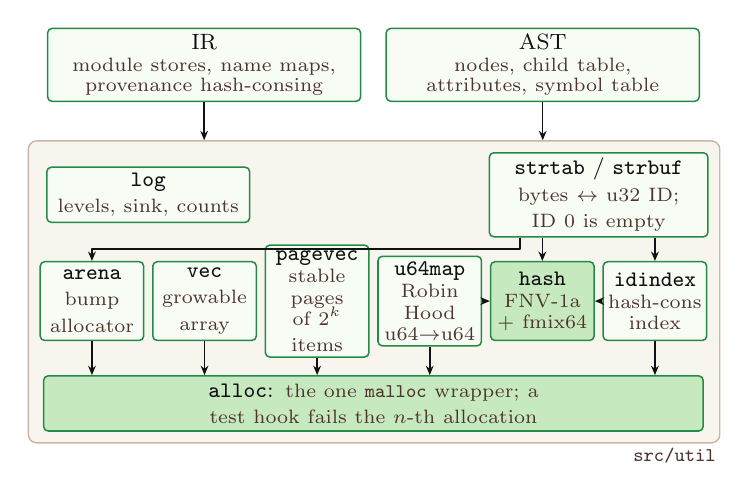
\begin{tikzpicture}[odin,
  c/.style={box, light, text width=12.3mm, minimum height=10mm, inner xsep=1.2pt},
  wide/.style={box, light, minimum height=7mm}]
  % ---- containers (tier 1) -----------------------------------------------------------------
  \node[c] (arena) at (0.667, 0) {\odintt{arena}\\\odinsub{bump allocator}};
  \node[c] (vec)   at (2.097, 0) {\odintt{vec}\\\odinsub{growable array}};
  \node[c] (pv)    at (3.527, 0) {\odintt{pagevec}\\\odinsub{stable pages\\[-2pt]of $2^k$ items}};
  \node[c] (u64)   at (4.957, 0) {\odintt{u64map}\\\odinsub{Robin Hood\\[-2pt]u64$\to$u64}};
  \node[c, fill=o3grn3] (hash) at (6.387, 0) {\odintt{hash}\\\odinsub{FNV-1a\\[-2pt]+ fmix64}};
  \node[c] (idx)   at (7.817, 0) {\odintt{idindex}\\\odinsub{hash-cons\\[-2pt]index}};
  % ---- foundation (tier 0) and strings / log (tier 2) ----------------------------------------
  \node[wide, fill=o3grn3, text width=82mm] (alloc) at (4.242, -1.3)
       {\odintt{alloc}: \odinsub{the one \odintt{malloc} wrapper; a test hook fails the $n$-th allocation}};
  \node[wide, text width=26mm] (str) at (7.102, 1.35)
       {\odintt{strtab} / \odintt{strbuf}\\\odinsub{bytes $\leftrightarrow$ u32 ID; ID 0 is empty}};
  \node[wide, text width=24mm] (log) at (1.382, 1.35) {\odintt{log}\\\odinsub{levels, sink, counts}};

  % ---- uses ----------------------------------------------------------------------------------
  \foreach \n in {arena, vec, pv, u64, idx} \draw[flow] (\n.south) -- (\n.south |- alloc.north);
  \draw[flow] (u64) -- (hash);
  \draw[flow] (idx) -- (hash);
  \draw[flow] (str.south -| hash) -- (hash.north);
  \draw[flow] (str.south -| idx) -- (idx.north);
  \coordinate (corr) at ($(str.south)!0.5!(str.south |- idx.north)$);
  \draw[flow] ($(str.south west)+(4mm,0)$) |- (corr -| arena) -- (arena.north);

  % ---- the users ---------------------------------------------------------------------------
  \begin{scope}[on background layer]
    \node[region, fit=(alloc)(arena)(idx)(str)(log), inner sep=4pt,
          label={[regionlabel, anchor=north east]south east:\odintt{src/util}}] (util) {};
  \end{scope}
  \node[box, light, text width=38mm] (ir) at (2.092, 3.0)
       {IR\\\odinsub{module stores, name maps,\\[-2pt]provenance hash-consing}};
  \node[box, light, text width=38mm] (ast) at (6.392, 3.0)
       {AST\\\odinsub{nodes, child table,\\[-2pt]attributes, symbol table}};
  \draw[flow] (ir.south) -- (ir.south |- util.north);
  \draw[flow] (ast.south) -- (ast.south |- util.north);
\end{tikzpicture}
}
\caption{\code{src/util}: the only generic containers in the tree, over one allocation wrapper
whose test hook fails the $n$-th allocation. Arrows point from a container to what it uses.}
\label{fig:util}
\end{figure}

\code{src/util} is the only place allowed to define a container (Fig.~\ref{fig:util}; 1A
spec). Containers are \code{void*} plus an element size, typed at the per-kind accessors,
rather than macro-generated (which hides control flow from the linters) or intrusive (which leaks
container fields into IR structs). \code{pagevec} stores pages of $2^k$ elements
($4 \le k \le 16$) behind a growable page table, so elements never move, lookup is a shift, a
mask and two loads, and growth never copies elements. Both hash tables use open addressing with
Robin Hood probing~\cite{celis1986robinhood} and backward-shift deletion. \code{idindex} is an
ID-only hash-cons index: its 16-byte slots hold a hash and an ID, and the caller supplies
equality, so interned strings and provenance records are stored once. String ID~0 is the empty
string, so a zeroed field means ``no name''. A bump \emph{arena} serves the small arrays that belong to one owner, such as parameter vectors,
wire net vectors and attribute values. Its blocks never move, and one call frees all of them.
The hash seed is a fixed constant; nothing that
reaches output depends on hash-map iteration order. A benchmark interned 2M names in
0.36--0.45\,s, made 2M \code{u64map} insertions in 0.35--0.39\,s and 2M \code{pagevec} pushes in
0.01\,s, at 176\,MiB maximum RSS.

\subsection{The IR}
\label{sec:ids}

\begin{figure*}[t]
\centering
\odinfit{\textwidth}{% Odin III IR object model (docs/IR.md sections 1-6, src/ir/ir_internal.h). Record sizes are
% sizeof() on x86-64 (gcc 13): node 40 B, pin 24 B, net 40 B, wire 40 B. Wide: \textwidth.
% Solid arrows are typed 32-bit ID references; double-headed arrows are the two directions of
% one relation; grey arrows are ownership.
\begin{tikzpicture}[odin,
  idref/.style={flow, draw=o3blue8},
  idref2/.style={idref, <->},
  owns/.style={flow, draw=o3grey6},
  lab/.style={edgelabel, fill=none, inner sep=1pt}]
  % ---- design and module -------------------------------------------------------------------
  \odinrecord{design}{anchor=north, nodes={text width=26mm},
              row 1/.style={nodes={fill=o3blue4}}, at={(1.39, 0)}}{Design}{
    strings (names, paths) \\ provenance store \\ pass-run table \\ tombstones \\
    cell-type table \\ modules[\,] \\ top \\}
  \odinrecord{module}{anchor=north, nodes={text width=31mm},
              row 1/.style={nodes={fill=o3blue4}}, at={(4.92, 0)}}{Module (IR-18)}{
    nodes: \odintt{pagevec} of node \\ pins: \odintt{pagevec} of pin \\
    nets: \odintt{pagevec} of net \\ wires: \odintt{pagevec} of wire \\
    name maps: \odintt{u64map} \\ alias, attribute side tables \\
    pin pool (sizes 2, 4, 8, \ldots) \\ arena (params, wire vectors) \\}
  % ---- per-module records ------------------------------------------------------------------
  \odinrecord{pin}{anchor=north, nodes={text width=27mm}, at={(8.70, 0)}}{pin \textmd{(24 B)}}{
    node: node ID \\ port, bit \\ net: net ID (0 = open) \\ slot in the net's pin array \\
    direction \\}
  \odinrecord{node}{anchor=north, nodes={text width=27mm}, at={(12.23, 0)}}{node \textmd{(40 B)}}{
    type: cell-type ID \\ name: string ID \\ prov: provenance ID \\ first\_pin, pin\_count \\
    params (in the arena) \\ dead flag \\}
  \odinrecord{net}{anchor=north, nodes={text width=27mm}, at={(8.70, -3.25)}}{net \textmd{(40 B)}}{
    pins[\,]: drivers, then sinks \\ driver\_count \\ name, prov \\ primary (wire, bit) \\
    alias chain \\ dead flag \\}
  \odinrecord{wire}{anchor=north, nodes={text width=27mm}, at={(12.23, -3.25)}}{wire \textmd{(40 B)}}{
    name, prov \\ {[}msb:lsb{]}, signed \\ nets[\,], LSB first \\ port node \\}
  % ---- design-wide records -----------------------------------------------------------------
  \odinrecord{ct}{anchor=north, nodes={text width=31mm}, row 1/.style={nodes={fill=o3grey3}},
              at={(15.96, 0)}}{cell type (IR-8)}{
    name: \odintt{\$add}, \odintt{\$\_AND\_}, \odintt{adder}, \ldots \\
    granularity: word, bit, hard, black box, module, port \\ ports and width rules \\
    params and defaults \\ hooks: verify, const\_value, simulate, writers \\}
  \odinrecord{prov}{anchor=north, nodes={text width=31mm}, row 1/.style={nodes={fill=o3grey3}},
              at={(15.96, -3.25)}}{provenance record (IR-12)}{
    kind: SOURCE, IMPORTED, DERIVED \\ pass run, operation \\ locations (file:line, raw) \\
    AST node ID \\ hierarchical path \\ parents[\,] \\}

  % ---- per-module storage region -----------------------------------------------------------
  \begin{scope}[on background layer]
    \node[bluregion, fit=(pin)(node)(net)(wire), inner sep=5pt,
          label={[regionlabel, anchor=south west]north west:per-module paged storage}] (store) {};
  \end{scope}

  % ---- ownership ---------------------------------------------------------------------------
  \draw[owns] (design-7-1.east) -- ++(0.35,0) |- (module-1-1.west);
  \draw[owns] (module-3-1.east) -- (module-3-1.east -| store.west);
  \draw[owns] (design-1-1.north) -- ++(0, 0.62) -| node[lab, above, pos=0.25] {cell-type table} (ct.north);
  \draw[owns] (design.south) -- (design.south |- 0,-7.15) -| node[lab, above, pos=0.25]
       {provenance store: append-only, hash-consed, design-wide} (prov.south);
  % ---- ID references -----------------------------------------------------------------------
  \draw[idref] (node-5-1.west) -- ++(-0.22,0) |- (pin-1-1.east);
  \draw[idref2] (pin-4-1.east) -- ++(0.2,0) |- (net-2-1.east);
  \draw[idref2] (wire-4-1.west) -- ++(-0.3,0) |- (net-5-1.east);
  \draw[idref] (node-2-1.east) -- ++(0.3,0) |- (ct-1-1.west);
  \draw[idref] (node-4-1.east) -- ++(0.45,0) |- (prov-1-1.west);
\end{tikzpicture}
}
\caption{The IR object model (IR.md). A module keeps nodes, pins, nets and wires in
per-kind paged arrays; every reference is a typed 32-bit ID (blue; double-headed arrows are the
two directions of one relation), and grey arrows are ownership. A node's pins are contiguous; a
net owns a contiguous pin array, drivers first. Record sizes are \code{sizeof} on x86-64.}
\label{fig:ir}
\end{figure*}

A design holds a string table, the provenance store, the cell-type table and its modules
(Fig.~\ref{fig:ir}). It also holds containers of facts that are not IR objects: the project
record and, since Phase~4.1, the \emph{arch record} that \code{read\_arch} fills from a VPR
architecture file (Sec.~\ref{sec:techlib}). A module owns nodes, pins and nets as peers, Odin~II's model: a node has
pins, a pin belongs to one node and attaches to one net, and a net has driver and sink pins.
A \emph{port} is not a separate kind of object. It is a node of a built-in type
(\code{\$port\_in}, \code{\$port\_out} or \code{\$port\_inout}), and a \emph{wire} is a name for an ordered
vector of nets. The same objects serve two granularities. In the word-level view, \code{assign y
= a + b;} on 8-bit signals is one \code{\$add} node with three ports of eight pins each. After
\code{lower}, the same eight-bit nets feed bit cells such as \code{\$\_XOR\_} and
\code{\$\_AND\_}. Only the node types change; the nets and the pins are the same kind of object.
The key decisions, numbered as in IR.md:

\emph{Every net is one bit (IR-1).} A port of width $w$ is $w$ consecutive pins, so a port is a
slice of its node's pins and word structure stays visible; word- and bit-level cells differ only
in type. Slicing and concatenation are which nets a pin vector uses, so there are no
\code{\$concat} or \code{\$slice} cells, and \code{lower}/\code{raise} replace cells without
splitting nets.

\emph{Wires are names, not connectivity (IR-2).} A wire is a named, ordered vector of nets with
a range and signedness. A net has at most one primary (wire, bit) and any number of aliases, so
\code{assign b = a;}, flattening and net merging keep every name.

\emph{Ports are nodes and constants are cells (IR-3, IR-4).} Each port is a \code{\$port\_in},
\code{\$port\_out} or \code{\$port\_inout} node, and constant bits come from shared constant
cells, so every driver is a pin and \code{check} has one driver rule.

\emph{Typed IDs, stable until \code{compact} (IR-5, IR-6).} Each kind has its own
\code{struct \{uint32\_t v;\}}, so the compiler rejects a net ID passed as a node ID; slot~0 is a
reserved dummy, so zero means ``none''. Deleting marks an object dead and keeps its slot.
\code{compact} renumbers live objects in ID order, frees dead slots and writes a tombstone per
dead object (module, kind, cell type, name, provenance, parameters, last connected net names) so
history still resolves.

\emph{Storage (IR-18).} Records are arrays of structs in per-module \code{pagevec}s: node
40\,B, pin 24\,B, net 40\,B, wire 40\,B. A throwaway spike (2M nodes, 4 pins each, 2.2M nets)
decided the layout: the whole IR took about 260\,MB, and a fanout walk took 2.8\,s with
intrusive linked pin lists, 0.85\,s with struct-of-arrays link fields and 0.24\,s with
contiguous per-net pin arrays. The net-to-pin representation, not AoS versus SoA, decides
traversal speed, so a net owns a pin array from a size-class pool (capacities 2, 4, 8,
\ldots), partitioned drivers-first so the driver lookup is O(1) and fanout is a slice.

\emph{Invariants (IR \S9).} \code{check} verifies eleven rules: pin ownership and index ranges,
pin--net agreement, the driver/sink partition, single drivers except declared tristate buses,
pin counts against port widths, unique names and agreeing name maps, valid provenance, wire
membership, port consistency, the granularity view, and dangling pins. The 1B benchmark on the
real implementation (2M nodes, 2.2M nets, each with a source record) measured build 0.835\,s,
full \code{check} 0.741\,s, fanout walk 0.313\,s, deleting 10\% 0.098\,s and \code{compact}
0.393\,s at 792\,MiB maximum RSS, inside the 2\,GB budget for Titan-scale designs.

\subsection{Op registry and cell types}

Each cell type is one table entry in one file (IR-8): name (Yosys spelling where one exists),
granularity, flags, ports with a width rule (a constant, an integer parameter, a function, or a
compiled expression supplied by the tech library), parameters with defaults, and hooks that may
be NULL: \code{verify}, \code{const\_value} (one predicate for ``is this net constant''),
\code{simulate} with its scratch-sizing hook, and writer hooks. Simulation flags distinguish
edge-triggered storage, which cuts the simulator's combinational graph, from level latches, which
do not. 75 types are built in. Phase~1 brought 53: ports, constants, the BLIF \code{\$sop} cover
and latch family, bit gates, and the word set (\code{\$add}, \ldots, \code{\$pmux},
\code{\$dff}, \code{\$mem}, \code{\$reduce\_*}). 2D-1 added nine Yosys simlib cells and
\code{\$proc}, 2E-1 eleven flip-flop and latch cells, and 3D-1 \code{\$lut}. The table is
append-only, so a built-in type's index never changes. Plugins register types at load time. Each module instantiates as a cell type of granularity \code{module} whose ports
mirror its port nodes, and each parameter specialisation is its own module (IR-7).

\subsection{Provenance}

\begin{figure}[t]
\centering
\odinfit{\columnwidth}{% Provenance lineage DAG (IR-12, IR-13), an illustrative example: one source line inside a
% generate loop elaborates to two $add cells (two SOURCE records, told apart by hier path);
% lowering each $add is one operation (one DERIVED record shared by its pieces); merging two
% gates is one operation with two parents. Records are immutable, hash-consed and design-wide;
% parents always have smaller IDs. Run and op numbers are illustrative. Single column.
\begin{tikzpicture}[odin,
  rec/.style={box, light, text width=21mm, minimum height=8.5mm},
  obj/.style={ellipse, draw=o3grey6, fill=white, line width=0.5pt, font=\scriptsize,
              align=center, inner xsep=-1pt, inner ysep=0pt, minimum height=6mm, text width=13mm},
  parent/.style={flow, draw=o3blue8},
  pid/.style={line width=0.5pt, draw=o3grey6, dash pattern=on 2pt off 1.4pt},
  band/.style={fill=o3grey1, draw=o3grey3, line width=0.4pt},
  bandlabel/.style={font=\scriptsize\bfseries, color=o3grey7, anchor=north west, inner sep=2pt}]
  % ---- run bands ---------------------------------------------------------------------------
  \foreach \y/\t in {0/{run 3: \odintt{read\_verilog}}, -1.58/{run 7: \odintt{lower}},
                     -3.16/{run 9: \odintt{opt}}} {
    \fill[band] (0, \y+0.72) rectangle (8.55, \y-0.86);
    \node[bandlabel] at (0, \y+0.72) {\t};
  }
  % ---- records -----------------------------------------------------------------------------
  \node[rec] (r1) at (3.0, -0.18)  {\#1 SOURCE\\\odinsub{\odintt{f.v:42}, \odintt{top/g[0]}}};
  \node[rec] (r2) at (5.55, -0.18)  {\#2 SOURCE\\\odinsub{\odintt{f.v:42}, \odintt{top/g[1]}}};
  \node[rec] (r3) at (3.0, -1.76) {\#3 DERIVED\\\odinsub{op 15}};
  \node[rec] (r4) at (5.55, -1.76) {\#4 DERIVED\\\odinsub{op 16}};
  \node[rec] (r5) at (4.275, -3.34) {\#5 DERIVED\\\odinsub{op 2, two parents}};
  % ---- IR objects --------------------------------------------------------------------------
  \node[obj] (a1) at (0.95, -0.2) {\odintt{\$add}\\[-1pt](dead)};
  \node[obj] (a2) at (7.6, -0.2) {\odintt{\$add}\\[-1pt](tombstone)};
  \node[obj] (g1) at (0.95, -1.76) {gates of\\[-1pt]\odintt{g[0]}};
  \node[obj] (g2) at (7.6, -1.76) {gates of\\[-1pt]\odintt{g[1]}};
  \node[obj] (g3) at (1.9, -3.34) {merged\\[-1pt]gate};
  % ---- edges -------------------------------------------------------------------------------
  \draw[parent] (r3) -- (r1);
  \draw[parent] (r4) -- (r2);
  \draw[parent] (r5.north) ++(-0.5,0) |- ($(r3.south)+(0,-0.3)$) -- (r3.south);
  \draw[parent] (r5.north) ++(0.5,0) |- ($(r4.south)+(0,-0.3)$) -- (r4.south);
  \foreach \o/\r in {a1/r1, a2/r2, g1/r3, g2/r4, g3/r5} \draw[pid] (\o) -- (\r);
  % ---- key ---------------------------------------------------------------------------------
  \begin{scope}[shift={(5.85, -3.6)}]
    \draw[parent] (0, 0.32) -- (0.45, 0.32);
    \node[font=\scriptsize, anchor=west, inner sep=1pt] at (0.5, 0.32) {parent};
    \draw[pid] (0, 0) -- (0.45, 0);
    \node[font=\scriptsize, anchor=west, inner sep=1pt] at (0.5, 0) {object's prov ID};
  \end{scope}
\end{tikzpicture}
}
\caption{The provenance lineage DAG (illustrative run and operation numbers). Two \code{\$add}s
from one line of a generate loop get two SOURCE records; lowering each is one operation with
one DERIVED record; clumping two gates is one operation with two parents.}
\label{fig:prov}
\end{figure}

Every node, net and wire carries one 32-bit provenance ID into an append-only, hash-consed
lineage DAG (Fig.~\ref{fig:prov}; IR-12, IR-13). A record holds its kind (SOURCE, IMPORTED from a
netlist, or DERIVED by a pass), the pass run and the operation number within that run, source
locations (file, line, column and the raw source-manager location from which macro and include
chains are derived on demand), the AST node, the hierarchical path, and parent records. The
run and operation fields are what keep lineage precise: without them, 100 \code{\$add}s from one
line of a generate loop would share a record and the gates their lowering produces would be
indistinguishable. Decomposing one object is one operation whose pieces share a record with a
single parent; clumping $N$ objects is one operation with $N$ parents; a pass that only rewires
keeps the records. Records are never edited or deleted, and provenance never names object IDs,
so \code{compact} cannot break lineage.

Navigation runs both ways without recursion. The backward walk visits the SOURCE and IMPORTED
leaves of a record. The forward index, built by one sweep over every live and dead object and
tombstone, answers ``everything that came from \code{foo.v:42}''. On the 2M-node benchmark it
was built in 0.064\,s (168\,MB), a query on the busiest line returned 200,000 hits in
0.341\,ms, and a backward walk over all 1.8M live nodes took 0.060\,s. Writers can name objects
\code{hier/path/cell@file:line}, so a VPR block can be traced to its source line without Odin III
loaded.

\subsubsection*{Provenance along the flow}

\begin{figure*}[t]
\centering
\odinfit{\textwidth}{% The flow annotated with the provenance records each stage makes. Wide: \textwidth.
\def\flowbandA{File names go into the source manager, one 32-bit location space for all files.}%
\def\flowbandB{Every AST node keeps a source range. Macro and include chains stay derivable
  from the location.}%
\def\flowbandC{No record is made.}%
\def\flowbandD{Each IR object gets a \textbf{SOURCE} record from its AST node. \odintt{proc}
  makes \textbf{DERIVED} records whose parent is the \odintt{\$proc} cell's record.}%
\def\flowbandE{Each pass opens a pass run. A rewrite is one operation with one \textbf{DERIVED}
  record; a merge has several parents. \odintt{flatten} stores the instance path. \odintt{fsm}
  parents the new state logic on the old.}%
\def\flowbandF{A hard block gets a \textbf{DERIVED} record with the word cell as parent. Nodes
  are named \odintt{cell.role}.}%
\def\flowbandG{Decomposing a word cell is one operation. The bit cells share one
  \textbf{DERIVED} record with the word cell as parent.}%
\def\flowbandH{One \textbf{DERIVED} record per LUT. Parents follow ABC's correspondence
  (\odintt{--prov fine} or \odintt{cone}).}%
\def\flowbandI{\odintt{--name-style provenance} writes names that end in \odintt{@file:line}. Plan
  5.4: \odintt{src} attributes in Verilog and JSON.}%
\def\flowbandJ{A reader makes an \textbf{IMPORTED} record per object. Plan 5.4 (IR-13
  amendment): one \textbf{DERIVED} record with the restored HDL \textbf{SOURCE} and the
  \textbf{IMPORTED} record as parents.}%
% The Odin III flow, drawn once (the O leg of tools/vtr-qor, qor_legs.py, plus the readers of
% Phase 5). Nine stages in two rows, a band of text under each box. The three figures that use it
% (fig_flow, fig_flow_verify, fig_flow_prov) define \flowbandA ... \flowbandJ, the text of each
% band, and then input this file. Wide figure: \textwidth.
\begin{tikzpicture}[odin,
  st/.style={box, built, text width=29.5mm, minimum height=13mm, inner ysep=2pt},
  band/.style={font=\scriptsize, text width=29.5mm, align=left, anchor=north, inner sep=1.2pt,
               color=o3ink}]
  % ---- row 1 ---------------------------------------------------------------------------
  \node[st] (s1) at (0, 0) {\textbf{Code}\\[-1pt]\odinsub{Verilog and the project}};
  \node[st] (s2) at (3.4, 0) {\textbf{Parse}\\[-1pt]\odinsub{\odintt{read\_verilog}: AST and symbol table}};
  \node[st, planned] (s3) at (6.8, 0) {\textbf{Before elaboration}\\[-1pt]\odinsub{no optimisation pass}};
  \node[st] (s4) at (10.2, 0) {\textbf{Elaborate}\\[-1pt]\odinsub{stage 1, stage 2, \odintt{proc}}};
  \node[st] (s5) at (13.6, 0) {\textbf{Word-level passes}\\[-1pt]\odinsub{\odintt{fsm}, \odintt{opt}, \odintt{flatten}, \odintt{wreduce}}};
  % ---- row 2 ---------------------------------------------------------------------------
  \node[st] (s6) at (0, -5.4) {\textbf{Partial mapping}\\[-1pt]\odinsub{\odintt{partial\_map} (\odintt{hardmap}) on the arch record}};
  \node[st] (s7) at (3.4, -5.4) {\textbf{Lower}\\[-1pt]\odinsub{\odintt{lower}: words to bits}};
  \node[st] (s8) at (6.8, -5.4) {\textbf{Logic and LUTs}\\[-1pt]\odinsub{linked ABC: \odintt{abc --lut K}}};
  \node[st] (s9) at (10.2, -5.4) {\textbf{Outputs}\\[-1pt]\odinsub{\odintt{write\_blif --vtr}, Verilog, JSON, LPM, dot}};
  \node[st, spec] (s10) at (13.6, -5.4) {\textbf{Read back}\\[-1pt]\odinsub{BLIF, Verilog, JSON readers (Phase 5)}};
  % ---- bands ---------------------------------------------------------------------------
  \foreach \i/\t in {1/\flowbandA, 2/\flowbandB, 3/\flowbandC, 4/\flowbandD, 5/\flowbandE,
                     6/\flowbandF, 7/\flowbandG, 8/\flowbandH, 9/\flowbandI, 10/\flowbandJ}
    \node[band] at ([yshift=-1.4mm]s\i.south) {\t};
  % ---- edges ---------------------------------------------------------------------------
  \foreach \a/\b in {s1/s2, s2/s3, s3/s4, s4/s5, s6/s7, s7/s8, s8/s9}
    \draw[flow] (\a) -- (\b);
  \draw[flow] (s5.east) -- ++(0.4,0) |- (0,-4.4) -- (s6.north);
  \draw[ref] (s9) -- (s10);
\end{tikzpicture}

}
\caption{The flow of Fig.~\ref{fig:flow}, annotated with the provenance records that each stage
makes or reads. SOURCE, DERIVED and IMPORTED are the three record kinds. The plan for Phase~5.4 is
shown where it applies; it is approved and not yet built.}
\label{fig:flow-prov}
\end{figure*}

Figure~\ref{fig:flow-prov} shows where each kind of record comes from. No stage builds a record by
hand. A pass runs with a context that knows its pass run, starts an operation, and asks for a
record with a list of parents (IR-13).

\emph{SOURCE, at parse and elaboration.} The parser gives every AST node a source range in the
source manager's location space. The read pass is a pass run. When elaboration creates an IR
object from an AST node, it makes one SOURCE record with the file, line and column, the raw
location and the AST node, and the object carries the record's ID. One origin in one run is one
record.

\emph{DERIVED, in each pass.} A pass makes a DERIVED record in one of three ways, depending on
what it does to the objects. A pass that only rewires keeps the existing records. A pass that
splits one object into many makes one operation and one record with the original as the single
parent. \code{proc}, \code{partial\_map} and \code{lower} work this way, so all bit cells of one
\code{\$add} share a record. A pass that joins several objects into one makes one operation whose
record has all of them as parents. \code{opt\_merge} works this way. \code{flatten} adds the
instance path to a DERIVED record, \code{fsm} gives the recoded state logic the original register
and logic as parents, and \code{abc} pairs each new LUT with the old cells that compute the same
function and takes those as parents. Records are never edited, and a deleted object leaves its
records and, after \code{compact}, a tombstone.

\emph{IMPORTED, on read.} A netlist reader has no HDL. It makes an IMPORTED record with the
file and line of the netlist, so that an object read from BLIF still says where it came from.

\emph{Names in the outputs.} With \code{--name-style provenance}, the writers name each object
\code{hier/path/name@file:line} from the first location of its backward walk, so a VPR block can
be traced to a source line without Odin III loaded.

\emph{Plan 5.4: locations survive write and read.} The IMPORTED record points at the netlist, not
at the HDL, so after a read-back the HDL location of a written object is lost. Phase~5.4 fixes
that. Writers print only the HDL locations, which are the SOURCE leaves of an object's walk:
the provenance name in BLIF, a \code{src} attribute in Verilog, and the \code{src} field in
JSON. Readers decode them. The architect approved an amendment to IR-13 on 2026-10-20: a reader
makes one DERIVED record whose parents are the restored HDL SOURCE record and the reader's own
IMPORTED record. The location then survives any number of writes and reads as an HDL location,
and a line of a netlist never becomes one. The coverage gate of Phase~6.5 measures the result.

\subsection{Source manager}

\begin{figure}[t]
\centering
\odinfit{\columnwidth}{% The source manager's location space for the worked example of the 2A spec section 3.1:
%   1  `define INNER(p) (p + 1)
%   2  `define OUTER(q) `INNER(q * 2)
%   3  assign y = `OUTER(xx);
% Buffers are allocated in creation order (F, E1, A1, E2, A2, A3) in one 32-bit location space,
% drawn left to right. Arcs above the strip: parent (where the buffer was entered); arcs below:
% def (where its bytes are spelled). Both always point to an earlier buffer. Single column.
\begin{tikzpicture}[odin,
  cell/.style={draw=o3grey6, line width=0.5pt, minimum height=9mm, align=center,
               inner sep=1pt, font=\footnotesize},
  kfile/.style={fill=o3blue4},
  kexp/.style={fill=o3blue2},
  karg/.style={fill=o3grey2},
  par/.style={flow, draw=o3blue8},
  def/.style={flow, draw=o3grey7, dash pattern=on 2.2pt off 1.3pt},
  arclab/.style={font=\scriptsize, fill=white, inner sep=0.8pt},
  seg/.style={draw=o3grey6, line width=0.5pt, minimum height=4.6mm, inner sep=1.5pt,
              font=\scriptsize, anchor=north west}]
  % ---- the strip: buffers in allocation order ----------------------------------------------
  \node[cell, kfile, minimum width=20mm] (F)  at (1.00, 0) {F\\\odinsub{\odintt{f.v}}\\[-2pt]\odinsub{lines 1--3}};
  \node[cell, kexp,  minimum width=13mm] (E1) at (2.65, 0) {E1\\\odinsub{OUTER}\\[-2pt]\odinsub{13 B}};
  \node[cell, karg,  minimum width=13mm] (A1) at (3.95, 0) {A1\\\odinsub{$q \leftarrow$ \odintt{xx}}\\[-2pt]\odinsub{2 B}};
  \node[cell, kexp,  minimum width=13mm] (E2) at (5.25, 0) {E2\\\odinsub{INNER}\\[-2pt]\odinsub{7 B}};
  \node[cell, karg,  minimum width=13mm] (A2) at (6.55, 0) {A2\\\odinsub{$p \leftarrow$ \odintt{xx}}\\[-2pt]\odinsub{2 B}};
  \node[cell, karg,  minimum width=13mm] (A3) at (7.85, 0) {A3\\\odinsub{$p \leftarrow$ \odintt{\textvisiblespace*\textvisiblespace2}}\\[-2pt]\odinsub{4 B}};

  % ---- parent arcs (above): apex height grows with the span --------------------------------
  \foreach \c/\p/\co/\po/\h/\l in {E1/F/-0.15/0.45/0.62/3:12, A1/E1/-0.15/0.12/0.62/E1+7,
                                   E2/E1/-0.3/0.36/1.3/E1+0, A2/E2/-0.15/0.12/0.62/E2+1,
                                   A3/E2/-0.3/0.36/1.3/E2+1}
    \draw[par] ($(\c.north)+(\co,0)$) .. controls +(0,\h) and +(0,\h) ..
          node[arclab, pos=0.5] {\l} ($(\p.north)+(\po,0)$);

  % ---- def arcs (below) --------------------------------------------------------------------
  \foreach \c/\p/\co/\po/\h/\l in {E1/F/-0.2/0.6/-0.62/2:18, A1/F/-0.2/0.3/-1.15/3:19,
                                   E2/F/-0.2/0.0/-1.68/1:18, A2/A1/-0.2/0.2/-1.15/A1+0,
                                   A3/E1/0.0/0.3/-2.2/E1+8}
    \draw[def] ($(\c.south)+(\co,0)$) .. controls +(0,\h) and +(0,\h) ..
          node[arclab, pos=0.5] {\l} ($(\p.south)+(\po,0)$);

  % ---- the preprocessed stream and its segment map -----------------------------------------
  \coordinate (s0) at (0.35, -2.95);
  \node[font=\scriptsize\bfseries, color=o3grey7, anchor=south west, inner sep=1pt] at (s0)
       {stream text and its segment map};
  \foreach \t/\l/\k/\w [count=\i, remember=\i as \j (initially 0)] in {
      {assign y =\textvisiblespace}/{F 3:1}/kfile/16.5mm,
      {(}/{E2+0}/kexp/8.6mm,
      {xx}/{A2+0}/karg/8.6mm,
      {\textvisiblespace*\textvisiblespace2}/{A3+0}/karg/10.6mm,
      {\textvisiblespace+\textvisiblespace1)}/{E2+2}/kexp/12.4mm,
      {;}/{F 3:22}/kfile/9.6mm} {
    \ifnum\i=1 \coordinate (at) at (s0); \else \coordinate (at) at (t\j.north east); \fi
    \node[seg, \k, minimum width=\w, font=\scriptsize\ttfamily] (t\i) at (at) {\strut\t};
    \node[seg, fill=white, minimum width=\w] (m\i) at (t\i.south west) {\strut\l};
  }
  \node[font=\scriptsize, color=o3sub, anchor=west, inner sep=1pt] at (m6.east) {\ location};
  \node[font=\scriptsize, color=o3sub, anchor=west, inner sep=1pt] at (t6.east) {\ text};

  % ---- key ---------------------------------------------------------------------------------
  \begin{scope}[shift={(0.35, -4.35)}, every node/.style={font=\scriptsize, anchor=west, inner sep=1pt}]
    \draw[kfile, draw=o3grey6] (0, -0.08) rectangle +(0.32, 0.22); \node at (0.36, 0.03) {FILE};
    \draw[kexp,  draw=o3grey6] (1.05, -0.08) rectangle +(0.32, 0.22); \node at (1.41, 0.03) {EXPANSION};
    \draw[karg,  draw=o3grey6] (3.15, -0.08) rectangle +(0.32, 0.22); \node at (3.51, 0.03) {MACRO\_ARG};
    \draw[par] (5.35, 0.03) -- +(0.4, 0); \node at (5.8, 0.03) {parent};
    \draw[def] (6.85, 0.03) -- +(0.4, 0); \node at (7.3, 0.03) {def};
  \end{scope}
\end{tikzpicture}
}
\caption{The location space for \code{`define INNER(p) (p + 1)},
\code{`define OUTER(q) `INNER(q * 2)} and \code{assign y = `OUTER(xx);}: buffers in allocation
order, left to right. Arcs above: where a buffer was entered (\emph{parent}); dashed arcs below:
where its bytes are spelled (\emph{def}); both point to earlier buffers. The segment map ties
each run of the preprocessed stream to a location.}
\label{fig:srcman}
\end{figure}

A location is one 32-bit offset into a virtual source space, as in Clang~\cite{clangsm}
(Fig.~\ref{fig:srcman}; 2A AST-1--AST-3). Buffers are allocated in creation order, each
reserving its length plus one: FILE buffers for source and project files (and a
\code{<command line>} buffer for project defines), an EXPANSION buffer per macro use, a
MACRO\_ARG buffer per contiguous spelled run of a substituted argument, and SCRATCH for pasted
text (Phase~5). Each buffer records its \emph{parent} (the macro use, the formal, the
\code{`include} or the project word that opened it) and its \emph{def} (where its bytes are
spelled). From these, three loops over buffer records give the spelling, the expansion location
(Clang's \code{getExpansionLoc}) and the file location, and a chain walk prints
``in argument of macro'', ``expanded from macro'' and ``included from'' lines. Each expansion
costs its body length once and each substitution its argument length once, so nesting does not
multiply space. The design owns the source manager, so provenance prints full chains for the
design's life while storing one 32-bit location per source record.

The preprocessor emits a \emph{segment map}: a new segment wherever the output stops following
the spelled bytes one for one, and a location-0 segment of its own for every inserted byte. The
lexer turns output offsets into locations with a monotone cursor. On \code{mcml.v} (650,837
bytes, 24,508 lines), location decode ran at 16.4\,M/s and the sequential cursor at 475\,M/s.
Preprocessing \code{mcml.v} produced 5,590 segments in 2,776 buffers and took 2.751\,ms (target
50\,ms) with a heap of 2.18 times the input; all 31 VTR benchmark files took 0.011\,s in total
at 4\,MiB maximum RSS (PHASE2 \#12).

\subsection{AST and symbol table}

\begin{figure}[t]
\centering
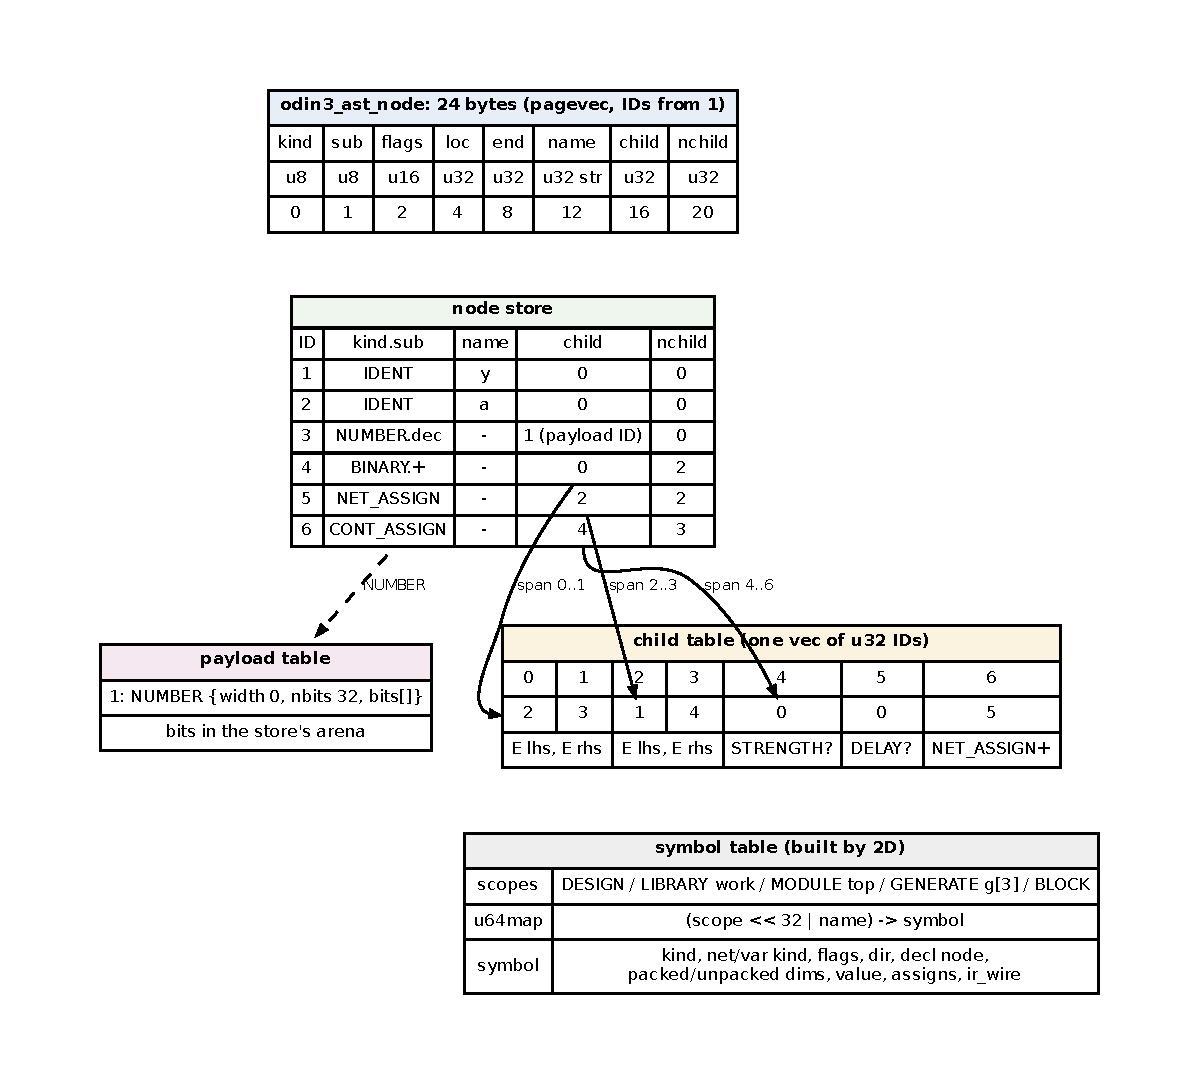
\includegraphics[width=\columnwidth]{fig_ast}
\caption{The 24-byte AST record (byte offsets above each field) and the stores for
\code{assign y = a + 1;}. Nodes are made bottom-up, so every child ID is below its parent's. Each
node owns one span of the shared child table (shaded alike); absent optional slots are ID~0;
literals live in a payload table.}
\label{fig:ast}
\end{figure}

The AST mirrors the IR's storage discipline (Fig.~\ref{fig:ast}; 2A AST-4--AST-16). A node is
24 bytes: kind and sub-kind (one byte each), 16 per-kind flag bits, a source range of two
32-bit locations, a string-table name, and a span (first index, count) into one shared child
table; payload kinds (numbers, reals, opaque text) reuse the span field as a payload index. A
normative \emph{slot table} fixes, for each of 68 kinds, its sub-kinds, whether it has a name,
its flags, its positional slots (absent optional slots are ID~0, so a slot's index never
moves) and its tail class and bounds; the builder validates every node against it, and
\code{check} verifies child classes. Nodes are built bottom-up, so every child ID is smaller
than its parent's: a forward sweep over IDs visits children first, and the store is
append-only and immutable once finished. Literals are stored as written and sized later
following Yosys's \code{read\_verilog} rules exactly. Comments go to a side table sorted by
location; attributes attach through a map from node to a span of attribute nodes.

A builder-enforced depth cap of 32,768 (ten times the deepest real expression found, a
2,032-term chain in Koios~\cite{arora2021koios} \code{lenet.v}) bounds every explicit stack.
On a synthetic 2M-node AST the store measured 41.17 bytes per node against a 40-byte target,
which was missed and relaxed (the 24-byte record plus number payloads); building took 0.101\,s,
a walk 0.015\,s and a full check 0.127\,s at 94,324\,KiB maximum RSS. A Verilog printer gives the
parser a parse--print--parse oracle.

The symbol table (AST-14) is a scope tree---design, one scope per library, one per module
specialisation, then generate (with loop index), block, function and task scopes---with one
\code{u64map} keyed \code{(scope << 32) | name} for Verilog's single namespace per scope.
Symbols record kind, net or variable kind, flags (signed, implicit, port, overridden, how
assigned), direction, declaration node, packed and unpacked dimensions, parameter value, every
assigning node, and the IR wire they became. ASTs and symbol tables are freed at the end of
their read pass unless a pass asks to keep them; SOURCE records keep the raw location either way.

The AST and the IR are separate stores, and a provenance record links them. When elaboration
creates an IR object from an AST node, it makes a SOURCE record that holds the node's ID, and the
object holds the record's ID. The AST is the high layer, with the syntax and the scopes. The IR is
the low layer, with cells and nets. The symbol table also points forward: each symbol records the
IR wire it became. A pass that needs the syntax of an object follows its record to the AST node,
if the store is still held. If it is not, the record still gives the file, line and column.

\subsection{Tech library and arch record}
\label{sec:techlib}

\begin{figure}[t]
\centering
\odinfit{\columnwidth}{% The tech library (1G spec): one .o3lib text format, read into design-local cell types whose
% port widths may be parametric and whose functions are expressions over the ports. The source
% is lib/vtr.o3lib's multiply cell, verbatim. Single column: \columnwidth.
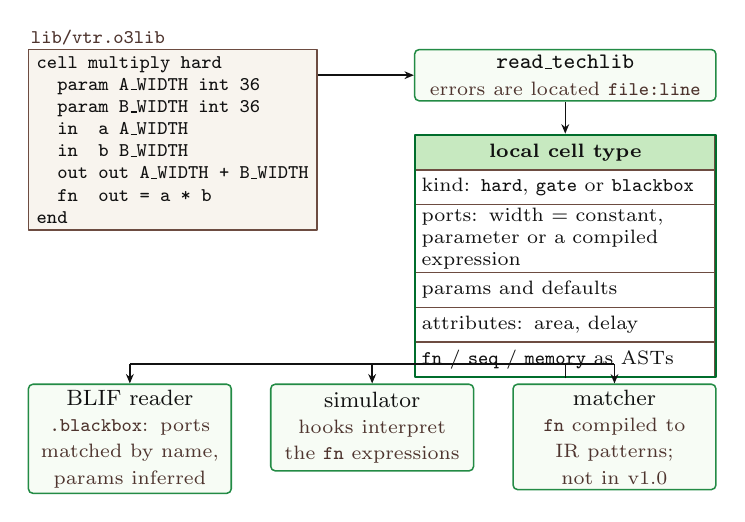
\begin{tikzpicture}[odin,
  fld/.style={draw=o3brn6, fill=white, line width=0.5pt, font=\scriptsize, align=left,
              text width=36.5mm, minimum height=4.4mm, inner xsep=2.2pt, inner ysep=1.2pt},
  use/.style={box, text width=24mm, minimum height=11mm}]
  % ---- source --------------------------------------------------------------------------------
  \node[draw=o3brn6, fill=o3brn1, line width=0.5pt, align=left, anchor=north west,
        inner xsep=3pt, inner ysep=2.5pt, font=\scriptsize\ttfamily,
        label={[font=\scriptsize\bfseries, color=o3brn7, anchor=south west, inner sep=1pt]
               north west:\odintt{lib/vtr.o3lib}}] (src) at (0, 0)
       {cell multiply hard\\
        \ \ param A\_WIDTH int 36\\
        \ \ param B\_WIDTH int 36\\
        \ \ in\ \ a A\_WIDTH\\
        \ \ in\ \ b B\_WIDTH\\
        \ \ out out A\_WIDTH + B\_WIDTH\\
        \ \ fn\ \ out = a * b\\
        end};
  % ---- reader and cell type ------------------------------------------------------------------
  \node[box, light, text width=36.5mm, anchor=north east] (rd) at (8.75, 0)
       {\odintt{read\_techlib}\\\odinsub{errors are located \odintt{file:line}}};
  \node[fld, fill=o3grn3, font=\scriptsize\bfseries, align=center, anchor=north]
       (h) at ($(rd.south)+(0,-0.42)$) {local cell type};
  \node[fld, anchor=north] (c1) at ($(h.south)+(0,\pgflinewidth)$) {kind: \odintt{hard}, \odintt{gate} or \odintt{blackbox}};
  \node[fld, anchor=north] (c2) at ($(c1.south)+(0,\pgflinewidth)$) {ports: width = constant, parameter or a compiled expression};
  \node[fld, anchor=north] (c3) at ($(c2.south)+(0,\pgflinewidth)$) {params and defaults};
  \node[fld, anchor=north] (c4) at ($(c3.south)+(0,\pgflinewidth)$) {attributes: area, delay};
  \node[fld, anchor=north] (c5) at ($(c4.south)+(0,\pgflinewidth)$) {\odintt{fn} / \odintt{seq} / \odintt{memory} as ASTs};
  \node[fit=(h)(c5), inner sep=0pt, draw=o3grn8, line width=0.7pt] (ct) {};
  % ---- users ---------------------------------------------------------------------------------
  \node[use, light, anchor=north west] (blif) at (0, -4.25)
       {BLIF reader\\\odinsub{\odintt{.blackbox}: ports matched by name, params inferred}};
  \node[use, light, anchor=north] (sim) at (4.375, -4.25)
       {simulator\\\odinsub{hooks interpret the \odintt{fn} expressions}};
  \node[use, light, anchor=north east] (pat) at (8.75, -4.25)
       {matcher\\\odinsub{\odintt{fn} compiled to IR patterns; not in v1.0}};
  % ---- edges ---------------------------------------------------------------------------------
  \draw[flow] (src.east |- rd) -- (rd.west);
  \draw[flow] (rd) -- (ct);
  \coordinate (rail) at ($(blif.north)+(0,0.25)$);
  \draw[line width=0.55pt, draw=o3ink] (ct.south) -- (ct.south |- rail);
  \draw[line width=0.55pt, draw=o3ink] (rail -| blif) -- (rail -| pat);
  \draw[flow] (rail -| blif) -- (blif.north);
  \draw[flow] (rail -| sim) -- (sim.north);
  \draw[flow] (rail -| pat) -- (pat.north);
\end{tikzpicture}
}
\caption{The \code{.o3lib} tech library: one text format (here the VTR \code{multiply} cell,
verbatim) read into local cell types whose widths may be parametric and whose functions are
expressions over the ports.}
\label{fig:techlib}
\end{figure}

The tech library is Odin III's own line-oriented text format, \code{.o3lib}
(Fig.~\ref{fig:techlib}; 1G spec), target-agnostic so that a flow can map to plain gates
first and FPGA targeting grows from the same format. Liberty is ASIC-timing-centric with no
word-level functions, genlib covers only combinational gates, and VPR XML has no functions and
keeps widths in \code{pb\_type}s, so importers for those formats would produce \code{.o3lib}
cells instead (VPR XML import is 4.1). A cell is \code{gate}, \code{hard} or \code{blackbox}; port widths may be integer
expressions over parameters (\code{A\_WIDTH + B\_WIDTH}); outputs are driven by \code{fn}
expressions, \code{seq} statements or a \code{memory} description; \code{area} and \code{delay}
are stored for later cost models. One function serves as simulation semantics today and, were a matcher built, as
its patterns compiled to IR fragments (D5, amended by D10: not in v1.0). A VPR architecture file reaches the same form through \code{read\_arch} (4.1). It reads the
\code{<models>} and \code{pb\_type}s into generic black-box cells of a tech library, and keeps what
\code{partial\_map} needs in the \emph{arch record}, a container on the design shaped like the
project record. The record owns no node, net, wire or ID. When a netlist declares a library cell
as a \code{.blackbox}, the reader matches its ports by name in any order and infers the
parameters from the declared widths: the goldens hold 49 distinct black-box stanzas whose port
order varies between files.

\subsection{C ABI and plugins}

\begin{figure}[t]
\centering
\odinfit{\columnwidth}{% The C ABI and plugin model (1D spec, DESIGN.md section 15.3, include/odin3/odin3.h ABI v4).
% Everything outside the core sees only odin3.h. Single column: \columnwidth.
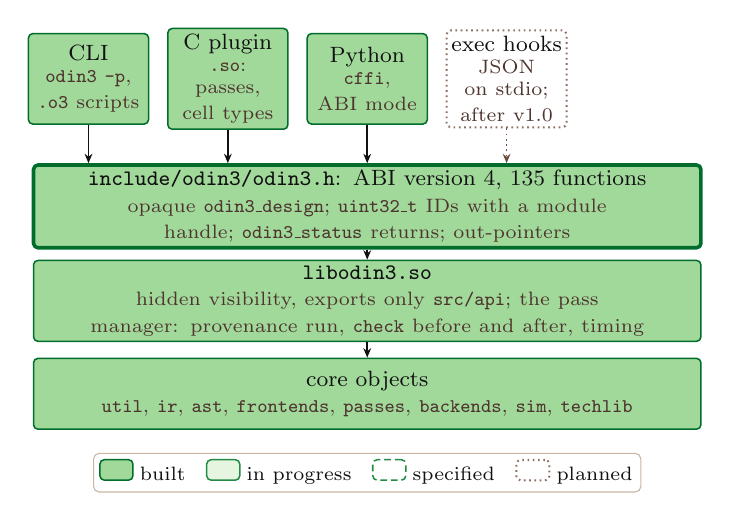
\begin{tikzpicture}[odin,
  client/.style={box, text width=14.2mm, minimum height=11.5mm, inner xsep=1.5pt},
  layer/.style={box, text width=83mm, minimum height=9mm}]
  % ---- clients -------------------------------------------------------------------------------
  \foreach \n/\x/\s/\t/\u in {
      cli/0.83/built/{CLI}/{\odintt{odin3 -p},\\\odintt{.o3} scripts},
      so/2.6/built/{C plugin}/{\odintt{.so}: passes,\\cell types},
      py/4.37/built/{Python}/{\odintt{cffi},\\ABI mode},
      hook/6.14/planned/{exec hooks}/{JSON on stdio;\\after v1.0}}
    \node[client, \s] (\n) at (\x, 0) {\t\\\odinsub{\u}};
  % ---- layers --------------------------------------------------------------------------------
  \node[layer, built, emph] (hdr) at (4.37, -1.62)
       {\odintt{include/odin3/odin3.h}: ABI version 4, 135 functions\\
        \odinsub{opaque \odintt{odin3\_design}; \odintt{uint32\_t} IDs with a module handle;
                 \odintt{odin3\_status} returns; out-pointers}};
  \node[layer, built] (lib) at (4.37, -2.82)
       {\odintt{libodin3.so}\\
        \odinsub{hidden visibility, exports only \odintt{src/api}; the pass manager: provenance
                 run, \odintt{check} before and after, timing}};
  \node[layer, built] (core) at (4.37, -4.0)
       {core objects\\
        \odinsub{\odintt{util}, \odintt{ir}, \odintt{ast}, \odintt{frontends}, \odintt{passes},
                 \odintt{backends}, \odintt{sim}, \odintt{techlib}}};
  % ---- edges ---------------------------------------------------------------------------------
  \foreach \n in {cli, so, py} \draw[flow] (\n.south) -- (\n.south |- hdr.north);
  \foreach \n in {hook}    \draw[flowplanned] (\n.south) -- (\n.south |- hdr.north);
  \draw[flow] (hdr) -- (lib);
  \draw[flow] (lib) -- (core);
  \odinlegend{anchor=north, at={(4.37, -4.75)}}
\end{tikzpicture}
}
\caption{The C ABI and plugin model. Everything outside the core sees only \code{odin3.h}.}
\label{fig:abi}
\end{figure}

An Application Binary Interface (ABI) is the contract between two pieces of compiled code. It
fixes the names of the functions, the types of their arguments and results, the sizes and layout
of the structures that cross the boundary, and the calling convention. An API describes this at the
source level, and a change that keeps an API can still break an ABI, for example by adding a field in
the middle of a structure. The ABI matters for plugins because a plugin is a separate compiled
object. A plugin built against one version of Odin III must still load and run against a later
build, without a recompile. A C ABI helps here, because C has no name mangling, no class layouts and
no exceptions that cross the boundary, and Python and other languages can call it. Odin III
therefore hides its internals, exposes only IDs and an opaque handle, versions the ABI, refuses a
plugin that asks for a different version, and keeps room in its structures for later hooks.

\code{include/odin3/odin3.h} is the only header plugins see (Fig.~\ref{fig:abi}; 1D spec,
DESIGN \S15.3). ABI version~4 declares its functions over an opaque design handle; IR objects
are raw 32-bit IDs passed with their module handle, every function returns
\code{odin3\_status} with results through out-pointers, NULL handles are rejected at the
boundary, and every declaration has a paragraph on purpose, ownership and failure modes.
\code{libodin3.so} is built with hidden visibility and exports only the definitions in
\code{src/api}; a script checks that the exported symbols equal the header's declarations.
Plugins are shared objects with an \code{odin3\_plugin\_init(abi\_version)} entry point that
registers passes and cell types (a mismatched ABI is refused); cell-type structs reserve hook
slots so later hooks do not break the ABI. Python uses the same header through cffi in ABI
mode, and executable hooks exchanging JSON are planned for Phase~7. Because the IR is IDs, the
ABI can hand them out safely and the IR serialises trivially.

\subsection{Caps and out-of-memory safety}

\begin{table}[t]
\caption{Selected resource caps (named constants, each a located error with a test). The
loop caps belong to elaboration (2D); all are built.}
\label{tab:caps}
\centering
\footnotesize
\begin{tabular}{@{}p{0.42\columnwidth}>{\raggedleft\arraybackslash}p{0.5\columnwidth}@{}}
\toprule
Cap & Value \\
\midrule
Reader port width / cell width & $2^{20}$ / $2^{22}$ bits \\
Source file / buffers per design & $2^{28}$ B / $2^{24}$ \\
AST depth / children per node & 32,768 / $2^{24}$ \\
Literal bits / decimal digits & $2^{20}$ / 4,096 \\
Include depth / expansion chain & 64 / 1,024 \\
Preprocessed stream & $2^{28}$ B \\
Parser stack (\code{YYMAXDEPTH}) & 262,144 \\
Errors per run (parser, elaboration) & 20 \\
Loop iterations: one / all & $2^{20}$ / $2^{24}$ \\
Byte budget (elaboration, \code{proc}) & smaller of 60\% of physical memory and the cgroup \code{memory.max} \\
\code{proc} pattern pool / reset rounds & $2^{24}$ bits / 100 \\
ABC script numbers / LUT inputs $K$ & $0..10^6$ / ${\le}\,12$ \\
\bottomrule
\end{tabular}
\end{table}

Every input-driven quantity has a named cap, checked before the allocation it guards and
reported as a located error (Table~\ref{tab:caps}). The motivation is practical: on the
development platform an out-of-memory condition kills the whole virtual machine (PHASE0 \#29),
and fuzzers produce macro, include and literal ``bombs''. A one-line BLIF \code{.subckt} must
not force gigabytes of pins; an exponential macro must stop at a stream, buffer or
location-space cap before memory runs out. Out of memory is a status, not a crash:
every container and IR operation reserves first, and unit tests fail every allocation in turn
through the \code{util} hook and assert that nothing changed and nothing leaked.

% ------------------------------------------------------------------------------------------
\section{Reverse Engineering}
\label{sec:re}

Reverse engineering was one of the three threads that started the project (DESIGN \S1): read a
flat netlist and recover the higher-level structure a designer would recognise. On 2026-10-19
the architect re-scoped v1.0 (ADR D10) and moved that thread. This section says what the goal
is now, what the built system already provides for it, what the removed Phase~6 design was, and
what open problems are left.

\subsection{The goal: from Altera all the way up}

The goal is now framed \emph{from Altera all the way up}. The architect's words (D10): ``we
will be looking reverse engineering from a different perspective of the goal of going from
altera all the way up \ldots\ I would like to target Altera devices with LPM and structured
verilog, but I'm not interested in their low-level formats.'' The start point is therefore Verilog that
Quartus-style flows produce or accept: a netlist of LPM megafunctions (\code{lpm\_add\_sub},
\code{lpm\_mult}, \code{lpm\_compare}, \code{altsyncram}) for Cyclone~V plus generic gates and
assigns. The end point is a higher-level description: word-level operators, memories and
registers, with every recovered object tied to the lines of netlist text it came from.
VQM and EDIF readers, device atoms (\code{stratixiv\_*}) and Titan are out of v1.0.

Phase~4.14, the Altera target, is the first step. Its LPM tech library (\code{.o3lib}) makes
such netlists \emph{readable}: the same library that lets a structural Verilog writer instantiate
LPM modules with their parameters lets the front end read them back, with each LPM instance
becoming a hard cell. An \code{lpm\_add\_sub} in the input is then already a word-level adder in
the IR, and a memory is an \code{altsyncram} hard cell, instead of an anonymous cone of gates.
The 4.14 test requires that the writer's output, re-read by the front end, gives the same
netlist with its LPM instances kept as hard cells (PHASE4). Recovering structure \emph{between}
the LPM cells (counters, shift registers, FSM state registers built from plain gates) is the
part that needs graph methods (Sec.~\ref{sec:re-graph}).

\begin{figure}[t]
\centering
\odinfit{\columnwidth}{% Reverse-engineering flow (paper section "Reverse Engineering"; D10, PHASE4 4.14, DESIGN 8, 12.1).
% Column width. Built = on main; specified = Phase 4.14 (planned, in PHASE4); planned = recorded
% in DESIGN 12.1 but removed from v1.0.
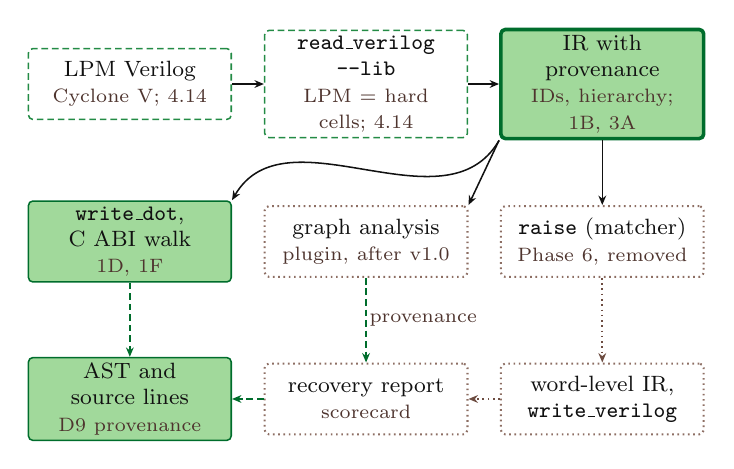
\begin{tikzpicture}[odin, node distance=3mm,
  box/.append style={minimum height=9mm, text width=24mm}]
  \node[box, spec]    (lpm)  at (1.25, 0)    {LPM Verilog\\\odinsub{Cyclone V; 4.14}};
  \node[box, spec]    (rd)   at (4.25, 0)    {\odintt{read\_verilog --lib}\\\odinsub{LPM = hard cells; 4.14}};
  \node[box, built, emph] (ir) at (7.25, 0)  {IR with provenance\\\odinsub{IDs, hierarchy; 1B, 3A}};

  \node[box, built]   (api)  at (1.25, -2.0) {\odintt{write\_dot}, C ABI walk\\\odinsub{1D, 1F}};
  \node[box, planned] (gra)  at (4.25, -2.0) {graph analysis\\\odinsub{plugin, after v1.0}};
  \node[box, planned] (raise) at (7.25, -2.0) {\odintt{raise} (matcher)\\\odinsub{Phase 6, removed}};

  \node[box, built]   (src)  at (1.25, -4.0) {AST and source lines\\\odinsub{D9 provenance}};
  \node[box, planned] (rep)  at (4.25, -4.0) {recovery report\\\odinsub{scorecard}};
  \node[box, planned] (wir)  at (7.25, -4.0) {word-level IR,\\\odintt{write\_verilog}};

  \draw[flow] (lpm) -- (rd);
  \draw[flow] (rd) -- (ir);
  \draw[flow] (ir) -- (raise);
  \draw[flow] (ir.south west) -- (gra.north east);
  \draw[flow] (ir.south west) to[out=-120,in=60] (api.north east);
  \draw[flowplanned] (raise) -- (wir);
  \draw[flowplanned] (wir) -- (rep);
  \draw[ref] (gra) -- node[edgelabel, right, fill=none] {provenance} (rep.north);
  \draw[ref] (rep) -- (src);
  \draw[ref] (api.south) -- (src.north);
\end{tikzpicture}
}
\caption{The reverse-engineering flow. Solid-blue boxes are built on main; dashed boxes are
the Phase~4.14 LPM path (planned, in PHASE4); dotted boxes are recorded designs that are not in
v1.0 (the plugin and \code{raise} routes). Dashed arrows are provenance links back to the AST
and source lines.}
\label{fig:re}
\end{figure}

\subsection{What already supports reverse engineering}

Provenance, identity and hierarchy were built for the forward flow, and they are the parts of
reverse engineering that cannot be retrofitted. Table~\ref{tab:re-support} lists them.

\begin{table}[t]
\caption{Built features that a reverse-engineering flow uses}
\label{tab:re-support}
\centering
\footnotesize
\begin{tabular}{@{}>{\raggedright\arraybackslash}p{0.24\columnwidth}%
  >{\raggedright\arraybackslash}p{0.50\columnwidth}p{0.08\columnwidth}@{}}
\toprule
Feature & Use & Phase \\
\midrule
Provenance (D9) & every object has a SOURCE or DERIVED record with a parents chain & 1B \\
Stable IDs & objects are 32-bit IDs, never pointers; a match can name its cells & 1B \\
Hierarchy and paths & dotted instance paths and \code{hier} kept in provenance &
  3A \\
\code{--lib} reads & library modules (such as an LPM definition) read as cells & 2C, 2D \\
Bit-node names & each gate named after the word cell it came from & 3B \\
Provenance names & \code{hier/path/name@file:line} in BLIF and Verilog & 3E-6, 1F \\
C ABI, Python walk & a plugin walks the IR and its provenance & 1D \\
Dot writer & Graphviz, focus on a cone, instance path or \code{file:line} & 1F \\
\bottomrule
\end{tabular}
\end{table}

\emph{Provenance (D9; IR-12, IR-13).} A record's kind is SOURCE, IMPORTED or DERIVED, and it
holds the pass run, the operation, the source location, the hierarchical path and the
\emph{parents}. Following the parents chain from a gate of the lowered netlist gives the word
cell it came from, and from there the AST node and the source line (Sec.~\ref{sec:data}). For
reverse engineering the same chain records what \emph{an analysis} decided: a recovered adder
would have as parents the gates that formed it. Netlists read from BLIF get structural-only
provenance until an analysis adds more (D9).

\emph{Stable IDs.} IR objects are 32-bit IDs in paged storage. \code{compact} renumbers them, but
provenance never names object IDs, so lineage survives. An analysis can hold a cell's ID safely
while it runs, and the C ABI hands out IDs, not pointers.

\emph{Hierarchy.} A design keeps its modules until \code{flatten} (DESIGN \S5.1).
\code{flatten} (3A) gives every object a dotted instance path (\code{u1.x}) and keeps the path in
the object's provenance, so a flat netlist still says which instance a gate came from. A
structure recovered from a flat netlist can be reported by instance.

\emph{Reads.} \code{read\_verilog --lib} reads module definitions as library cells (3C's
\code{hardmap-diff} reads its n-bit adder this way), and \code{read\_blif} reads BLIF with black
boxes into the same netlist view. \emph{Names.} \code{lower} names bit nodes after their word
cell (3B, PHASE3 \#38), and \code{write\_blif --vtr --name-style provenance} and
\code{write\_verilog --name-style provenance} print \code{hier/name@file:line}, so a name read in
a netlist leads to a source line.

\emph{Walk and view.} A plugin, in C or in Python through cffi, walks nodes, nets and
provenance through the ABI (1D exit test: ``a Python plugin walks the IR''). \code{write\_dot}
draws a cone, an instance or all objects from a source line, and refuses to draw more than a node
budget without a focus, so a large netlist stays readable.

\subsection{The removed Phase 6 design: \code{raise}}

The original plan, recorded now in DESIGN \S12.1, had one engine with two directions
(DESIGN \S8; D5). \emph{Forward}, the subgraph matcher binds cells to hard blocks. \emph{Backward}
it runs as \code{raise}: ``RE is literally \code{lower} run backwards''. Bit-level cones are
replaced by word-level cells, and the result is written as higher-level Verilog.

\emph{The matcher.} VF2-style subgraph matching~\cite{cordella2004vf2}, with three additions.
\emph{Anchor seeding}: candidates start at anchor cells instead of at every node (forward, a
\code{\$mul}). \emph{Width-agnostic} patterns: a pattern says ``an adder
of any width'', and the width is read from the matched cone. \emph{Local equivalence}: before a
candidate is committed, ABC proves the cone equal to the word-level cell that would replace it,
on the cone alone, so a wrong match cannot enter the IR (D4).
Overlapping candidates are resolved by maximum cover with a cost tie-break.

\emph{Structures to recover.} Ripple and carry-lookahead adders, comparators, mux trees,
counters, shift registers, memories, and FSM state registers.

\emph{Scorecard and round trip.} The test is a round trip: Verilog, \code{lower}, BLIF, read,
\code{raise}, Verilog, equivalence check. A structure-recovery scorecard counts how many
structures of a known design the pass finds (DESIGN \S11). The Titan subset, smallest first, was
the scale test (Phase~6.6).

All of it is out of v1.0 (D10, DESIGN \S12.1): the matcher (D5 amended; 4.10 dropped),
\code{raise} (6.1), the scorecard (6.2), VQM and EDIF readers (6.3), Altera \code{bind} (6.4),
the primitive library (6.5) and Titan (6.6). The reasons are that Verilog is good enough, that
the Altera work that matters is LPM structural Verilog, and that a matcher would add a pattern
language and scale risk to a tool whose goal is to work. Until then, hard blocks are matched by
exact port signature and the fixed 3C rules.

\subsection{Graph analysis: the architect's vision}
\label{sec:re-graph}

The architect's vision for reverse engineering is graph methods on the netlist: find the
high-level structure of a flat structural Verilog netlist by analysing its graph, and link every
result back to the AST through provenance, so that a recovered block points at lines of source
and the result can inform downstream decisions. The structures in view are datapaths, FSMs,
register files, counters and bus groupings. Subgraph matching, above, is one such method. Which
other graph methods to use is not decided (Sec.~\ref{sec:re-open}). This paper reports the
\emph{hooks} that the core keeps for them, not results:
\begin{itemize}
\item provenance on every object and an append-only parents chain, so an analysis can add
  records without rewriting any;
\item stable IDs, hierarchy paths and the instance structure, so results are reported by
  instance;
\item the C ABI and Python plugins that walk the graph, and the registry that lets a plugin add
  cell types for the structures it finds;
\item the netlist and word-level views, so a recovered word-level cell can sit among bit cells
  (IR-9 allows mixed granularity only inside \code{lower} and \code{raise}).
\end{itemize}
The route after v1.0 is the one the architect named: add techniques through libraries and
plugins, without changing the core. D10's last rule protects that route: IR provenance, IDs,
hierarchy and the C ABI stay intact, so a matcher, \code{raise} and other analyses can be added
later as plugins.

\subsection{Open problems}
\label{sec:re-open}

\begin{enumerate}
\item \emph{What is recoverable from LPM?} LPM hides the carry chain and the memory port logic
  inside the megafunction. How much structure the surrounding gates still show, and how to name
  it, is open. The 4.14 write-and-reread test shows only that a netlist Odin III wrote can be
  read back.
\item \emph{Which structures first?} Counters and shift registers are small cycles, and FSM
  state registers need state recoding to be undone (Yosys's \code{fsm} one-hot recoding is the
  forward direction, and it is out of v1.0). The order is undecided.
\item \emph{How to score.} The scorecard needs designs with known structure. Round-tripping
  Odin III's own output is circular, so it needs designs from outside.
\item \emph{Equivalence at scale.} Local equivalence per candidate needs ABC on cones, and
  \code{dsec} already gives ``unproven'' on several large designs (Sec.~\ref{sec:verify}).
\item \emph{Naming.} Recovered structures need names that mean something. Provenance names
  point to source lines, and a netlist from Quartus has none that carry intent.
\item \emph{Which graph methods.} Which graph methods beat subgraph matching on structural
  netlists, and for which structures, is a research question this paper does not answer.
\item \emph{The plugin interface.} An analysis plugin needs to add cells and provenance records
  safely. Phase~7's extension-API review is where that interface is checked.
\end{enumerate}

% ------------------------------------------------------------------------------------------
\section{Comparison with Yosys and Odin II}
\label{sec:compare}

\begin{table*}[t]
\caption{Odin II, Yosys (with Parmys) and Odin III compared}
\label{tab:compare}
\centering
\footnotesize
\begin{tabular}{@{}p{0.15\textwidth}p{0.25\textwidth}p{0.25\textwidth}p{0.28\textwidth}@{}}
\toprule
 & Odin II (VTR) & Yosys + Parmys & Odin III \\
\midrule
Core language & C-style code, built as C++ & C++ & C17; C++ only in adapters \\
Netlist & pointer graph: nodes hold pin-pointer arrays, nets hold driver and fanout pin pointers &
  RTLIL: wires and cells in name-keyed dictionaries; connections are SigSpecs of wire slices &
  per-module paged records; typed 32-bit IDs; one-bit nets; net-owned pin arrays \\
Granularity & bit-level netlist & word-level cells and processes; bit-level after techmap &
  one IR, word and bit views (Sec.~\ref{sec:arch}) \\
AST & \code{ast\_node\_t} with pointer children, \code{\{file, line, col\}} & \code{AstNode}
  with owned children, attribute map & 24-byte records, ID spans, slot table, 32-bit locations \\
Provenance & AST pointer on nodes; names & \code{src} attribute (\code{file:line.col}) &
  lineage DAG on every node, net and wire, with macro and include chains \\
Traversal & recursive (e.g.\ expression reduction) & recursive (e.g.\ AST simplification) & iterative only; capped \\
Resource limits & implicit & implicit & named caps; OOM is a status \\
Input & command line, XML config & scripts, command line & project record: \code{.o3proj},
  \code{-f}, Quartus; includes architecture and mapping rules \\
Architecture & VPR XML hard blocks & Parmys reads VPR XML & \code{.o3lib} (VPR XML import: 4.1) \\
ABC & separate step in the VTR flow & external process with a script & default script in a
  linked \code{libabc}; other scripts checked, then run in a capped child process; script
  SHA-256 recorded \\
SV / VHDL & no & yosys-slang, GHDL plugins & slang adapter at the seam; GHDL (deferred, D10) \\
Simulator & yes & \code{sim}, \code{eval}, SAT-based passes & yes, registry semantics \\
Extension & source changes & C++ passes and plugins & C ABI \code{.so}, Python cffi \\
License & MIT (VTR) & ISC & MIT \\
\bottomrule
\end{tabular}
\end{table*}

Table~\ref{tab:compare} summarises the differences. Yosys is the more complete and more mature
tool by a wide margin, with a pass library, formal flows and language coverage Odin III will not
match for years; Odin~II pioneered architecture-aware hard-block mapping for VTR. The
differences below are choices made for Odin III's research goals and its development method,
not claims of general superiority.

\emph{C17, a lint gate and no recursion.} The core is structured C17 (ADR D8$'$), replacing an
earlier C++20 plan, for five reasons: code an agent writes and a human reviews in one pass,
a stable language-neutral plugin boundary, ABC being C, the Odin~II lineage, and complexity
that a linter can enforce. The gate is blocking in pre-commit and CI: clang-format, clang-tidy, cppcheck, lizard
(cyclomatic complexity at most 15, functions at most 60 lines and 5 parameters), a rules script
(no \code{exit} outside the CLI, no \code{abort} outside \code{check}, \code{goto} only to a
single \code{cleanup:} label), \code{-Wvla} under \code{-Werror}, and ASan with UBSan on every
unit test. Recursion is
banned in traversals because the IR can be 2M nodes deep; Yosys's AST simplification and Odin
II's expression reduction are recursive, which is reasonable for hand-written RTL but is a stack
risk for machine-generated designs such as Koios's 2,032-term chains.

\emph{IDs and paged storage instead of pointer graphs.} RTLIL's SigSpec, a list of wire slices
per connection, is expressive but makes every rewrite split slices; Odin~II's pointer graph
makes serialisation and safe external handles hard. Odin III's one-bit nets with contiguous
pin arrays keep rewiring a matter of pin moves, give O(1) drivers and slice fanout, make
\code{compact} and the ABI straightforward, and cost little: the spike measured 260\,MB for 2M
nodes. The price is per-bit storage for wide buses, which the 2M-node benchmarks show is within
budget.

\emph{Provenance as a first-class structure.} Yosys keeps a \code{src} string attribute that
passes propagate where they choose; Odin~II keeps a pointer to the AST node that made a netlist
node. Neither records which pass made an object from which others. Odin III's lineage DAG
records every decomposition and clump, survives deletion through tombstones, and is queried in
both directions, because the research threads need it: reverse engineering reports which
netlist region became which recovered structure, mapping explains which rule chose a binding,
and a user can trace a VPR block to a source line.

\emph{Explicit caps and OOM safety.} Section~\ref{sec:data} explains the caps. Neither Yosys
nor Odin~II defines input-driven limits; both rely on the host. For a tool meant to be fuzzed
and run unattended on shared machines, a located error is better than a killed process.

\emph{Project files carry the architecture and the ABC script.} Odin~II took an architecture
file and an XML configuration; Yosys takes scripts. Odin III makes the project the unit of
reproducibility: sources, defines, top and parameters, the architecture with its inventory and
research overrides, the mapping rules, and the flow. The architect's decision for Phase~3 extends
this to ABC: the project file names the ABC script (\code{abc\_script <file>} in
\code{.o3proj}), \code{--abc-script} on the command line overrides it, and the \code{abc} pass
records the script's path and SHA-256 in its run record, so a soft-logic experiment is recorded
with the design rather than in a wrapper script.

\emph{Linked ABC for the vetted script, a sandbox for the rest.} Yosys's \code{abc} pass writes
the netlist to a per-run temporary directory and runs ABC on it, in a child process or, in builds
with ABC linked, in-process; VTR runs ABC as a separate flow step. ADR~D3 links ABC instead (its permissive license allows linking into the MIT core),
so the \code{abc} pass can hand ABC the soft-logic cone in memory, keep black boxes and
provenance, and stitch the LUTs back. The 3D-0 spike gave a go for the in-memory exchange
(MiniAIG in, MiniLUT out) on two micros, a hand-made \code{scorr} input and five Parmys goldens:
every LUT had at most six inputs, \code{dsec} proved each result equivalent, every register name
mapped back (0 state mismatches in a 256-cycle lockstep simulation), 1,000 runs in one process
gave identical results with no leaked bytes, and two processes gave the same hash (PHASE3
\#22). Linking has a price that a child process does not: ABC calls \code{exit} and
\code{abort}, asserts, and dies on some options, and in-process it takes the IR with it. The
script checker (3D-4) therefore parses every script against an allow-list built from ABC's
sources at the pin, with its 112 aliases, and refuses file, process and latch commands and a
fourth class: options that crash the pinned ABC. Its audit is the finding that decided the
design (PHASE3 \#27). About 70,000 runs of the pinned \code{abc} over six rounds did not
converge. Every round that tried new design shapes, $K$ values or option values found new crash
classes, because ABC's asserts and unchecked allocations depend on the design as much as on the
options. The guard catches an assertion only on the session thread, nothing in a Release
\code{libabc}, and no runaway output (\code{print\_kmap} on a 20-input node prints $2^{20}$ cells).
The architect's ruling (PHASE3 \#28) splits the difference. The built-in default script, the
eight logic commands VTR's ABC stage runs every day, runs in-process through the linked engine.
Any other script, from \code{abc --script}, \code{--abc-script} or the project, still passes the
checker and then runs in a child \code{abc} process with a wall-clock limit and an output cap,
and a crash or timeout there fails that run, not \code{odin3}. The checker, the SHA-256 identity
and the run record are the same on both paths. Odin III thus keeps linking where it is safe and
measured, and pays for isolation only where the input is untrusted.

\emph{Yosys~0.55 semantics as the oracle, with declared divergences.} Rather than reinterpret
IEEE~1364-2005~\cite{ieee1364} independently, Odin III adopts the semantics of the Yosys inside
Parmys (0.55) as its oracle for literal sizing, widths and signedness, parameter precedence and
process generation, and checks against it through \code{write\_rtlil} and equivalence checking.
Where it differs, the difference is declared and tested: the 2D specification lists 24
divergences (for example, automatic top selection requires a single uninstantiated module,
\code{\$readmem} files are never searched in the working directory, and unconnected inputs are
driven by \code{x}), and the preprocessor declares its own (for example, directives inside
macro text are errors, recursion is judged on the spelling ancestry, and includes never search
the working directory). Parity yields to correctness in one place so far (2E \S20 \#18,
confirmed by the architect in PHASE2 \#16). When a \code{casez} group ends on a path that
builds no cell, Yosys~0.55's \code{proc\_mux} keeps the mux open, and the next group's case
appends to a mux that no longer reaches the result, so its value is lost. For
\code{casez (s) 2\textquotesingle b00: y=x0; 2\textquotesingle b01: y=a; 2\textquotesingle b??: y=a; k: y=b;} Yosys gives $y = a$ where
Verilog gives \code{x0} for $s = 00$. A \code{miter}/\code{sat} check finds the
counterexample, Yosys's own \code{eval} of its netlist disagrees with the source, and Icarus
gives Verilog's value. 2E ends the open mux and gives Verilog's value; \code{proc-diff} and an
equivalence check against a Parmys golden flag such inputs, with 2E on the correct side.
Odin~II is kept as a read-only reference: a coverage audit of 159 synthesizable Verilog-2005
constructs~\cite{ieee13641} (100 required, 25 recommended, 10 ignored, 24 rejected) probed
Odin~II and Yosys with about 340 one-module tests and found constructs Odin~II's grammar lacks
(e.g.\ \code{casez}, attributes, ANSI function headers) and constructs it elaborates
differently from Yosys (e.g.\ dropped signedness), shown with equivalence checking.

\emph{The elaboration seam.} Yosys gains SystemVerilog by translating slang's elaborated design
into RTLIL inside a plugin; Odin~II has no SV path. Odin III's seam
(Fig.~\ref{fig:seam}) puts the shared work---widths, signedness, drivers, memories,
processes---in one stage~2 that both the Verilog stage~1 and the slang adapter feed, so the
(deferred) Phase~5 test that three front ends give one netlist would have one place to fail.

\emph{Agentic, spec-first development with oracles.} Odin~II and Yosys grew through human
contributions. Odin III is written by AI coding agents under an architect's control, so its
correctness evidence must come from outside the code: golden BLIFs from Parmys and Odin~II on
two architectures (2,380 oracle runs: 1,846 succeeded, 522 failed and 12 hit the memory cap),
\code{netlist-compare} (canonicalised identity), \code{equiv-check} (ABC \code{cec}/\code{dsec}),
a differential preprocessor check against Icarus Verilog~\cite{icarus} and Yosys, the project
corpus, and fuzzers. Section~\ref{sec:method} describes the method.

% ------------------------------------------------------------------------------------------
\section{Development Methodology}
\label{sec:method}

Every sub-project follows the same path: a specification in \code{docs/specs} with numbered
decisions, an independent critique by a fresh read-only agent, an implementation plan, tasks
dispatched to implementer agents with disjoint files and a written interface, a critique of every
pull request before it opens, and a merge only on a green CI gate (PHASE0 \S A.1). Decisions are
logged per phase; the architect makes or reviews every design-rule decision (specification, ADRs,
IR invariants, mapping algorithms), in some phases after the fact, and the agent proceeds on its
own recommendations elsewhere, logging each as a default he may override. Exit tests are external: the Phase~1 BLIF round trip
ran over every successful golden, the simulator was compared cycle by cycle with Icarus running
an independent dump of the same netlist, and the writers were validated through Yosys.

Review is layered. A controller agent owns git and dispatches each plan task to an implementer
agent, which may not dispatch agents of its own. A fresh reviewer then reads the task's diff and
reports findings graded critical, important or minor; the implementer fixes them in numbered
fix rounds, and an important finding gets a re-review. Before a pull request opens, a
whole-branch review reads the entire branch against its specification and plan, on a different
model (Fable) where one is available, else Opus at extra-high effort. The spec reviews were graded the same way; the 2D
specification's first review, for example, raised 2 critical, 10 important and 17 minor
findings, all applied before approval (PHASE2 \#13). Commit messages name each round and the
findings it answers, so the history records why each fix was made.

Several agents share one 24\,GB WSL virtual machine, and an out-of-memory condition there kills
the whole machine (PHASE0 \#29). Every heavy job (a benchmark sweep, a long fuzz run, VPR)
therefore goes through \code{tools/heavy-run}: a machine-wide lock admits one heavy job at a
time, and the job runs in a systemd slice capped at 6\,GiB with no swap (9\,GiB for the few
jobs that need it), so a runaway job is killed alone. Nesting is decided from the job's cgroup
and the inherited lock descriptor, never from environment variables alone, because a review
found that a leaked variable could let a job run uncapped. Sweeps are CTests registered so that \code{heavy-run}
alone decides whether they may run.

Cost is logged from the agents' transcripts (\code{docs/log\_cost\_of\_tokens\_and\_time.md}).
From 2026-10-08 16:15 to 2026-10-11 19:29 UTC (75.2\,h wall clock, 30.4\,h active), 10,922 API
requests used 2.47 billion tokens, 96\% of them prompt-cache reads, across 6 main sessions and
227 subagent runs: 9,198 requests to Claude Opus~5.5, 1,088 to Sonnet~5.5, 618 to Fable~5.1 and
18 to Haiku~5.5. \todo{regenerate the token log to cover 2026-10-12 and later at submission
time}

% ------------------------------------------------------------------------------------------
\section{Status and Roadmap}
\label{sec:status}
\begin{table*}[t]
\caption{Development phases (DESIGN \S12 as amended by ADR D10) and status on 2026-10-19}
\label{tab:phases}
\centering
\footnotesize
\begin{tabular}{@{}p{0.03\textwidth}>{\raggedright\arraybackslash}p{0.28\textwidth}%
  >{\raggedright\arraybackslash}p{0.26\textwidth}>{\raggedright\arraybackslash}p{0.19\textwidth}%
  >{\raggedright\arraybackslash}p{0.13\textwidth}@{}}
\toprule
Ph. & Deliverable & Exit test & Status & Target \\
\midrule
0 & environment, oracle builds, golden BLIFs, \code{netlist-compare}, \code{equiv-check}, lint
  gate, CI & oracles green on all goldens & done & --- \\
1 & \code{util}, IR, op registry, pass manager, \code{check}, provenance, C ABI, BLIF I/O,
  writers, simulator, tech library & BLIF$\to$IR$\to$BLIF identical; simulation matches ABC; a
  Python plugin walks the IR & done & --- \\
2 & Verilog-2005 front end, preprocessor, elaboration, project input, \code{proc}, \code{opt} &
  micros equivalent to Parmys; project fixtures elaborate from each format & done, closed
  2026-10-18 (PHASE2 \#30) & --- \\
3 & \code{wreduce}, \code{flatten}, \code{lower}, \code{hardmap}, linked ABC,
  \code{write\_blif --vtr}, QoR harness & the 19 VTR~7.0 benchmarks through place and route
  with Odin III alone; QoR table against Parmys & built; M1 met; Parmys-matching refinements,
  3D-7 default flip, 3D-8 and the M2 and M3 exit runs in progress & before Phase~4 closes \\
4 & \emph{the tool works on VTR architectures and on Altera via LPM}: VPR-XML import, generic
  hard blocks, multiplier and memory splitting, carry chains, FF features, memory port merge,
  Cyclone~V LPM target (4.14) & VTR designs route on several architectures and pass
  \code{fcheck}; LPM netlist equivalent to the RTL; QoR parity is not a gate & planned (PHASE4)
  & v1.0 about 5--10 Nov \\
5 & slang adapter (SystemVerilog), GHDL path (VHDL) & none in v1.0 & deferred: Verilog is close
  enough; nothing built & after v1.0 \\
6 & \code{raise}, RE scorecard, VQM and EDIF, Altera \code{bind}, Titan & none in v1.0 &
  removed from v1.0; design kept in DESIGN \S12.1 (Sec.~\ref{sec:re}) & --- \\
7 & CIRCT writer, Yosys JSON reader, visual tooling, documentation with the extension-API
  review, release (EDIF writer dropped) & release & planned & with v1.0 \\
\bottomrule
\end{tabular}
\end{table*}

Table~\ref{tab:phases} lists the phases. The status comes from the repository's phase
documents and from the measured runs of 2026-10-19 that Sec.~\ref{sec:measured} reports. The
v1.0 scope is ADR D10, accepted on 2026-10-19: ``since our goal is to make Odin III \ldots\ I
just want the tool to work.'' That moves QoR parity with Parmys out of the exit criteria
(it is still measured and reported), and it defers or removes the work that was not needed to
make the tool work. Section~\ref{sec:v1plan} gives the reasons item by item. The target date
is the controller's estimate; Phase~3 must close first.

Phase~1's exit tests passed on the goldens: every one of
the 1,846 successful golden BLIFs read and wrote back identically under the text gate, and 1,824
were also identical under \code{netlist-compare} (10 with stub models for implicit cells), with
the remaining 22 being 4 multi-driver Odin~II originals the comparator refuses and 18 comparator
timeouts or memory-cap stops on the largest Odin~II netlists; the reader and writer handled the
915\,MB \code{LargeRam} netlist in 16.8\,s. The simulator matched the reference on all 1,626
simulated goldens (4 of them after rerunning the reference simulator with a longer timeout;
220 excluded: 206 with RAMs, 10 implicit black boxes, 4 multi-driver), the
JSON writer was identical through Yosys on 1,796 goldens, structural Verilog was equivalent on
1,428 with none non-equivalent, and the Python walk agreed with the C \code{stats} pass on all 141
committed fixtures.

Phase~2 has built the source manager, AST and symbol table (2A), and the project readers and
preprocessor (2B), whose differential check against Icarus and Yosys over 287 files gave 271
agreements, 11 cases where the two oracles disagree (all as expected), 5 declared divergences and
20 excluded files (headers read only through another micro), with no differences or crashes. The
Odin~II XML reader (2B-4) completed project input.

The parser (2C) is built (PHASE2 \#15). Its sweeps run \code{odin3-parse-check}, with the
location oracle and the print and re-parse round trip, on every file, smallest first. Of 539
micros, 489 pass and 50 are expected failures, each listed with its reason, and each also
rejected by Parmys; there are no unexpected failures. All 64 VTR and Koios benchmarks pass, in
7.5\,s. Writing the 1,846 golden BLIFs as Verilog and parsing them back succeeds on 1,840; the
other 6 are 317\,MB to 2.1\,GB of Verilog and stop at the source-file cap, by design. Parsing
\code{mcml.v} (650,837 bytes, 78,229 nodes) takes 0.020\,s, and its AST and source manager take
4.56\,MB (targets 1\,s and 20\,MB); the 31 VTR files take 0.085\,s in total. Koios
\code{lenet.v} (11\,MB, 919,695 nodes) reads in 0.221\,s at 75,416\,KiB peak RSS. The parser
declares its divergences: it is stricter than Parmys's \code{read\_verilog -sv} on forms
outside Verilog-2005 (SystemVerilog named-argument calls and \code{.*}, a \code{casez}
generate) and more lenient on \code{macromodule}, which Yosys lacks. The architect has ruled that a stray \code{;} module item be accepted
with a warning, as Yosys and Icarus accept it (PHASE2 \#16).

Phase~2 is closed (PHASE2 \#30, 2026-10-18). Elaboration (2D), \code{proc} (2E) and \code{opt}
(2F) are merged, and the exit harness (2H) compared the micros and the VTR set with Parmys.
Of the 14 small VTR designs used as the equivalence evidence set, 9 are proved equivalent to
Parmys and 5 are untested (\code{diffeq1}, \code{diffeq2}, \code{mkPktMerge}, \code{sha} and \code{blob\_merge}: the SAT proof
reaches its size limit, so they are carried to a bigger machine; the big designs are moved to the
Phase~3 exit). On random processes, the \code{proc} mux phase gave
netlists identical to Yosys~0.55's on 547, and the other 6 made Yosys fail an assertion
(\code{ctrl\_sig.size() == 1}) on valid input that 2E lowers (\S20 \#17). The review of the
open-mux fix (\S20 \#18) found 2E byte-identical to Yosys on 319 of 330 random processes, in the
same normal form on 4 more, and \code{sat}-equivalent on all 323 that Yosys lowers. 2D's targets
are \code{mcml.v} in at most 0.5\,s and Koios \code{lenet.v} in at most 10\,s, against
Yosys~0.55's measured 0.48\,s and 14.3\,s
\todo{measured 2D elaboration results on mcml.v and lenet.v}.

\begin{table}[t]
\caption{The first Parmys baseline (leg P) through \code{vtr-qor} on
\code{k6\_frac\_N10\_frac\_chain\_mem32K\_40nm}, against VTR's golden results (PHASE3 \#25)}
\label{tab:qor}
\centering
\footnotesize
\begin{tabular}{@{}lr@{}}
\toprule
Measure & Value \\
\midrule
Jobs with \code{vpr\_status=success} & 21 of 21 \\
Wall time, 18 jobs (3 reused from cache) & 1\,h 08\,m 46\,s \\
Parmys BLIF byte-identical to the golden & 21 of 21 \\
\midrule
\multicolumn{2}{@{}l}{\emph{Geomean of P/golden over the 19 (the 2 extras: 1.000)}} \\
CLBs (\code{num\_clb}) & 1.000 \\
Minimum channel width $W$ & 0.995 \\
Critical-path delay & 1.000 \\
Routed wirelength & 1.001 \\
Designs equal to the golden on all four & 16 of 19 \\
\midrule
\multicolumn{2}{@{}l}{\emph{Peak memory (\code{LU32PEEng}; ABC: \code{mcml})}} \\
VPR & 2,264\,MiB \\
Parmys & 1,186\,MiB \\
VTR's ABC stage & 364\,MiB \\
\bottomrule
\end{tabular}
\end{table}

Phase~3's exit test runs the 19 VTR~7.0 benchmarks on
\code{k6\_frac\_N10\_frac\_chain\_mem32K\_40nm} with Odin III alone producing each netlist
(the script of Sec.~\ref{sec:backend}), routes them with VPR, passes VTR's functional check, and
reports a QoR table against the Parmys flow with a loose gate: a geomean ratio of at most
1.20, and no design above 1.50, on CLB count, channel width, critical-path delay and routed
wirelength. The gate compares the decimals VTR prints exactly, so 1.20 passes and 1.2001 fails.
Its milestones are M1 (the P$'$ leg routes all 19), M2 (the O$'$ leg routes all 19) and M3
(the O leg routes all 19, the exit).

The harness's first run of the Parmys leg (Table~\ref{tab:qor}; PHASE3 \#25) routed all 21
designs (the 19 plus \code{arm\_core} and \code{spree}, as VTR's \code{vtr\_reg\_qor\_chain}
task runs them), with nothing capped or timed out. The 18 jobs it started took 1\,h 09\,m,
against a planned 4 to 4.5\,h; the three smallest were reused from an earlier run. Its geomeans match VTR's golden results to within 0.5\%, and no metric is outside VTR's
pass bands. The three designs that differ do so in channel width: \code{diffeq2} 68 against 58,
\code{diffeq1} 50 against 62, and \code{LU8PEEng} 84 against 88. Peak VPR memory, 2,264\,MiB,
is far below the 6\,GiB heavy-run cap. The architect has approved publishing the baseline to
the golden repository and ruled out nightly QoR runs (PHASE3 \#28): the sweeps once planned for
a nightly run go through \code{heavy-run}, started by hand, before the PRs that need them
merge.

\subsection{Measured results, 2026-10-19}
\label{sec:measured}

Table~\ref{tab:measured} lists the results measured by the controller's runs on 2026-10-19
(each is a recorded run, with its command and log in the phase documents).

\begin{table*}[t]
\caption{Measured results on 2026-10-19 (the controller's runs; phase and sub-phase in the first column)}
\label{tab:measured}
\centering
\footnotesize
\begin{tabular}{@{}>{\raggedright\arraybackslash}p{0.12\textwidth}%
  >{\raggedright\arraybackslash}p{0.82\textwidth}@{}}
\toprule
Phase & Result \\
\midrule
2 (2H) & 14 small VTR designs: 9 proved equivalent to Parmys, 5 untested (size limit). \\
3B \code{lower} & \code{lower-gen-diff}, 200 seeds: 200 ok. 5,000 seeds: 4,830 ok, 142 structural,
  28 empty, 0 bugs. \\
3C \code{hardmap} & 12 big VTR designs: every hard-cell and flip-flop count difference against
  Parmys is explained. The causes are \code{fsm} recoding, the flip-flop-bit merge, the
  \code{wreduce} order and \code{opt\_share}. None comes from a mapping rule. \\
3H \code{fcheck} & Odin III's O-leg netlists of \code{sha}, \code{blob\_merge} and \code{or1200}
  pass 50,000 random vectors, where the Parmys netlists fail. The cause is the Parmys subtract
  padding defect (D2b). \\
3D-7 \code{abc-diff} & 29 k6 goldens: every design that finished is equivalent across the BLIF
  and in-memory exchanges. LUT ratios are 0.95 to 1.02 (\code{sha} 1.077). \\
M1 & the P$'$ leg routes all 19 VTR designs with VPR. \\
\bottomrule
\end{tabular}
\end{table*}

The \code{lower} generator is the broadest check of 3B: the two runs give no bug, and the 142
structural seeds are proved equivalent to the source with a one- or two-gate histogram difference
from Yosys's \code{techmap} (Sec.~\ref{sec:verify}). The \code{hardmap} result says the hard-block
\emph{rules} (3C) reproduce Parmys's, and that what remains of the count differences belongs to
passes that run before it. The \code{fcheck} result is the reverse of the usual direction: Odin
III's netlists are right and Parmys's are wrong, because of the divergence D2b (Sec.~\ref{sec:verify}).

\subsection{In progress and next}

Five items are open. (1) \emph{Parmys matching.} The flip-flop-bit merge, the \code{wreduce}
operand-first order and \code{opt\_share} parity are being made to match Parmys, since the
explanations above are the only source of count differences. (2) \emph{The in-memory ABC
exchange.} PR~148 adds it (3D-7); flipping it to the default and 3D-8 follow. (3) \emph{M2 and
M3.} The O$'$ and O exit runs, with the QoR table and gate, run when the lanes are idle, since a
running sweep holds the machine-wide heavy lock. (4) \emph{Name style.} The cost of provenance
names in VPR (the Oprov leg) is not measured yet. \todo{Odin III (leg O) against the Parmys
baseline once M3 runs} (5) \emph{The token log.} It is regenerated at the end of a session.

\subsection{The v1.0 plan and what was deferred or removed}
\label{sec:v1plan}

Phase~4, ``the tool works'' (PHASE4), keeps: VPR-XML import (4.1); generic hard blocks matched by
exact port signature (4.2); multiplier splitting from the architecture (4.3); memory depth and
width splitting (4.4); carry chains from the architecture's model (4.5); flip-flop feature
matching (4.6); memory port merge (4.7); the architecture sweep (4.13); and the Altera target
(4.14). The sweep runs the VTR designs on \code{k6\_frac\_N10}, one DSP architecture and one
plain-LUT architecture (which ones is an open item). The Altera target is Cyclone~V (Quartus
Lite), with exactly four LPM cells (\code{lpm\_add\_sub}, \code{lpm\_mult}, \code{lpm\_compare}
and \code{altsyncram}, single- and simple-dual-port) and plain D flip-flops in soft logic (an
agent default); everything else is generic structural Verilog. Its test is that the LPM netlist
is equivalent to the RTL under the LPM simulation models.

\begin{itemize}
\item \textbf{Dropped from Phase~4}: FSM detect and recode (4.8), because the tool works without it
  (it is the cause of the flip-flop count differences that the 3C row of
  Table~\ref{tab:measured} explains); mux collapsing (4.9), already done by \code{opt\_muxtree}
  and \code{opt\_reduce}; the matcher (4.10, D5 amended); project mapping rules (4.11), which the
  project still reads and stores; per-bit \code{opt\_dff} parity (4.12), since QoR parity is no
  longer a goal.
\item \textbf{Phase~5, deferred}: SystemVerilog through slang and VHDL through GHDL. Verilog-2005 is
  close to good enough, and nothing is built. DESIGN \S12.1 records how each step would be done.
\item \textbf{Phase~6, removed}: the reverse-engineering work of Sec.~\ref{sec:re}. Reverse
  engineering is now approached from Altera LPM up, which 4.14 starts.
\item \textbf{Phase~7, kept}: the CIRCT writer, the Yosys JSON reader, visual tooling, documents
  with the extension-API review, and the release. The EDIF writer is dropped.
\end{itemize}
The decision is to be revisited if the architect reopens reverse engineering or Titan, if
Verilog-only input proves too limiting, or if exact-port-signature matching cannot cover a block
that the VTR sweep needs (D10).

% ------------------------------------------------------------------------------------------
\section{Conclusion}

Odin III is a research front end designed around three needs that existing tools serve only in
part: architecture and mapping rules carried with the design, lineage from every netlist object
back to its source and through every transformation, and a core simple and checked enough for
AI agents to build and a human to review. Its IR keeps Odin~II's node/pin/net model in ID-based
paged storage; its front end follows Yosys's semantics, declaring every divergence; and its
elaboration seam prepares one back half for Verilog and SystemVerilog alike. As of 2026-10-19
the whole forward flow is built: \code{proc}, \code{opt}, \code{wreduce}, \code{flatten},
\code{hardmap}, \code{lower}, linked ABC and \code{write\_blif --vtr}, with a QoR harness that
reproduces VTR's own Parmys baseline. Each stage is checked by a tool that is separate from the
code, under an exit-code discipline in which a listing never counts as a pass. Where Odin III's
netlists differ from Parmys's in function, the measured cause so far is a Parmys padding defect,
not an Odin III one. The next milestones are the Parmys-matching refinements and the M2 and M3
exit runs, then Phase~4: VTR architecture sweeps and the Cyclone~V LPM target, which is also
the first step of reverse engineering from Altera upward. Provenance, stable IDs, hierarchy and
the C ABI are kept intact, so that matcher-based and graph-based analyses can be added after
v1.0 as libraries and plugins without changing the core.
\todo{QoR summary once the Phase 3 exit runs (M3) finish}

\section*{Acknowledgment}
\todo{acknowledgments and funding}

\bibliographystyle{IEEEtran}
\bibliography{odin3}

\end{document}
